\documentclass{book}
\usepackage{palatino}
\usepackage{graphicx}

\usepackage{fancyhdr}
%\usepackage{fullpage}
\usepackage{alltt}
\usepackage{url}
\usepackage{fancyvrb}

\def\summary#1{{\em#1}}
\def\caveat#1{
  \begin{center}
    \begin{tabular}{|p{10cm}|}
        \hline
        \noindent \bf Caveat: \em#1 \\
        \hline
    \end{tabular}
  \end{center}}
\def\apitype#1#2{{~\\\noindent\bf Type \tt{#1}}\\{#2}}
\def\apifunction#1#2{{~\\\noindent\bf Function \tt{#1}}\\{#2}}

\setlength\headsep{0.4cm}
\setlength\parindent{0cm}

\title{Man metalua 0.4}

\author{Fabien {\sc Fleutot}\\[10mm] 
  $-\left\{\begin{minipage}{7.6cm}
      \hspace{3mm}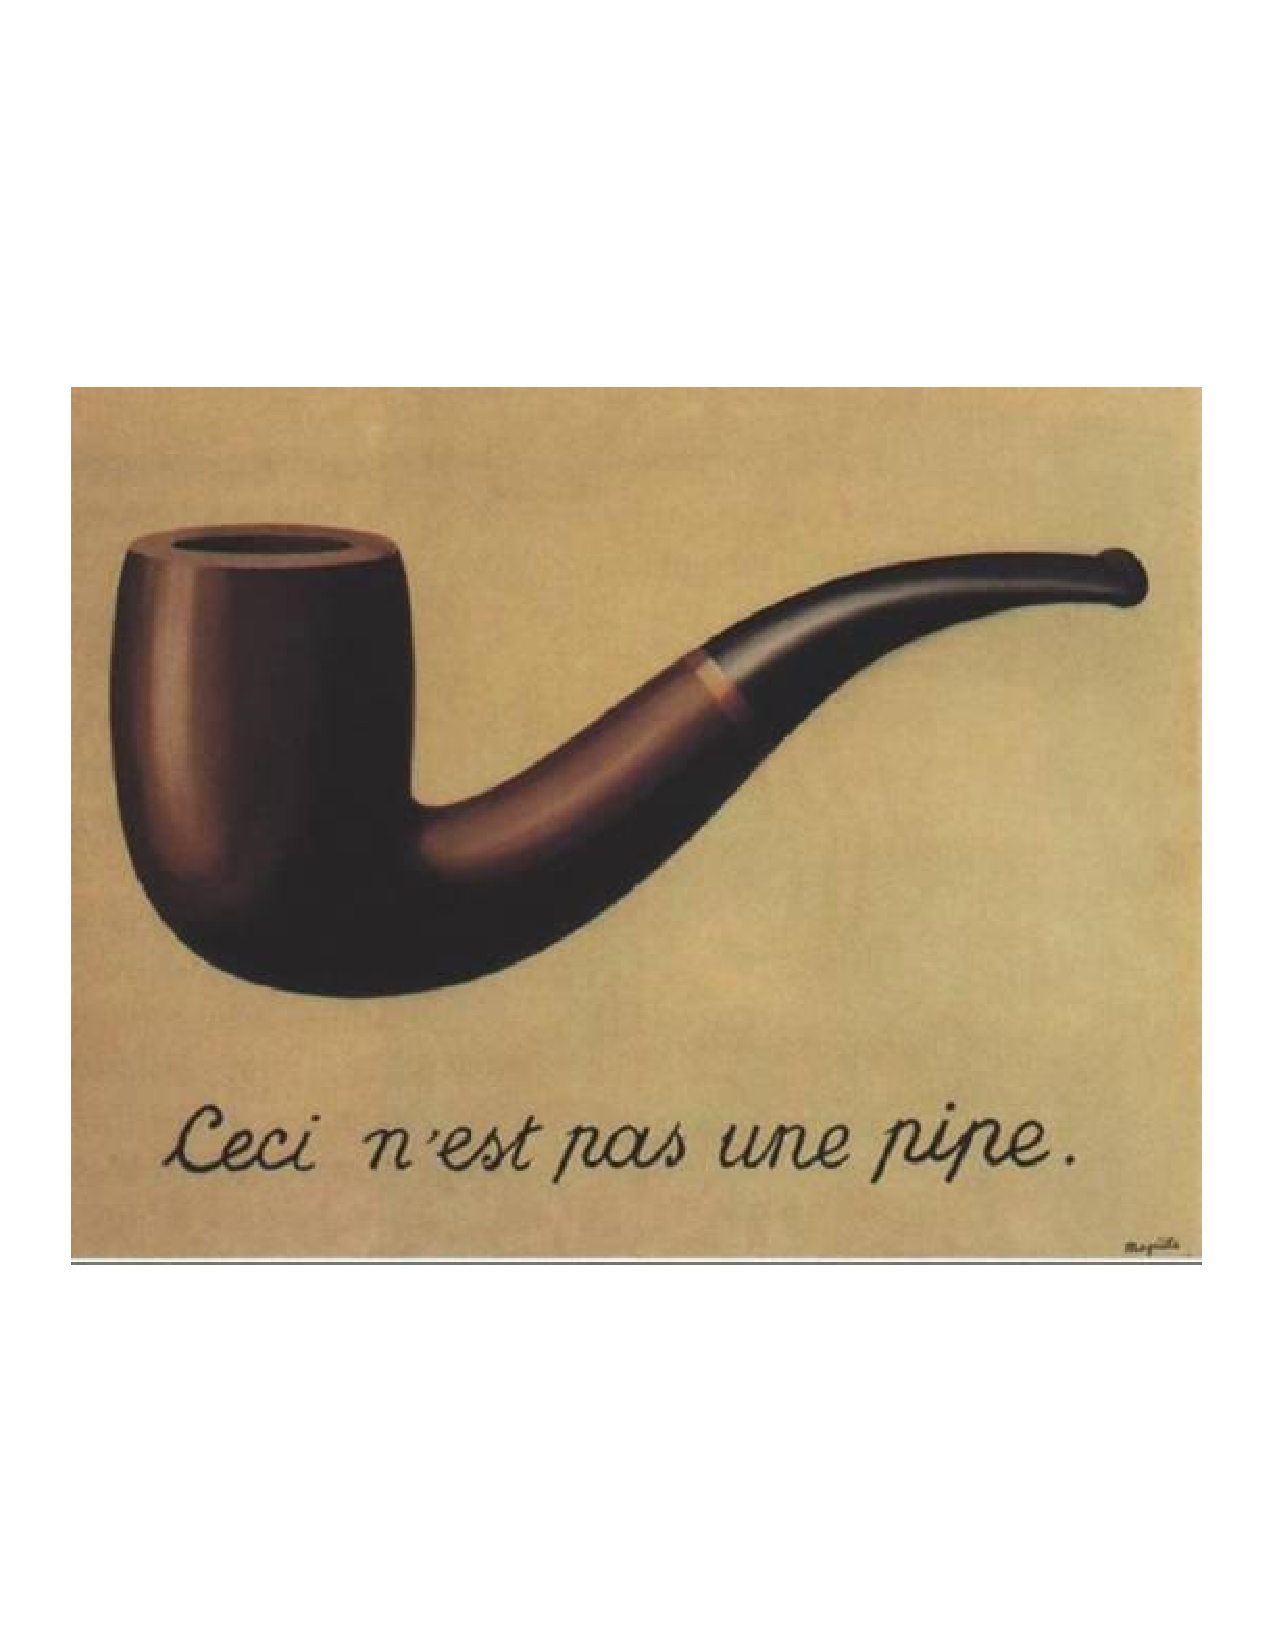
\includegraphics[width=7cm]{magritte.pdf}
    \end{minipage}\right\}$}

\begin{document}

\pagestyle{fancy}
\setlength\parskip{0.2cm}

\maketitle
\section*{Reading guide}
This manual tries to be as comprehensive as possible; however, you don't
necessarily have to read all of it before starting to do interesting stuff with
metalua. Here's a brief summary of what the different parts of the manual
address, and why you might want to read them immediately---or not.

\begin{itemize}
\item{\bf Before reading this manual:} metalua is based on Lua, so
  you'll need a minimal level of Lua proficiency. You can probably get
  away without knowing much about metatables, environments or
  coroutines, but you need to be at ease with basic flow control,
  scoping rules, first-class functions, and the whole
  everything-is-a-table approach.
\item{\bf Meta-programming in metalua:} this chapter exposes the generic principles
  of static meta-programming: meta-levels in sources, AST representation of
  code, meta-operators. You need to read this carefully if you plan to write any
  non-trivial meta-programming code and you've never used languages like, Common
  Lisp, camlp4 or Converge. If you're familiar with one of these, a cursory look
  over this chapter might be enough for you.
\item{\bf Standard meta-programming libraries:} these are the tools that will allow
  you to manipulate code effectively; the more advanced an extension you want to
  write the more of these you'll want to know.
  \begin{itemize}
  \item{\bf mlp} is the dynamically extensible metalua parser. You need to know it
    if you want to change or extend the language's syntax
  \item{\bf gg} is the grammar generator, the library which lets you manipulate
    dynamic parsers. You need to know it in order to do anything useful with
    mlp.
  \item{\bf match} is an extension supporting structural pattern matching (which has
    almost nothing to do with regular expressions on strings). It's a construct
    taken from the ML language familly, which lets you manipulate advanced data
    structures in vrey powerful ways. It's extremely helpful, among others, when
    working with AST, i.e. for most interesting meta-programs.
  \item{\bf walk} is a code walker generator: smomething akin to a visitor pattern,
    which will help you to write code analysers or transformers. Whenever you
    want to find and transform all return statements in an AST, rename some
    conflicting local variables, check for the presence of nested for loops
    etc., you'll have to write a code walker, and walk will get you there much
    faster. 
  \item{\bf hygiene} offers hygienic macros, i.e. protects you from accidental
    variable captures. As opposed to e.g. Scheme, macro writing is not limited
    to a term rewriting system in metalua, which lets more power to the
    programmer, but prevents from completely automating macro hygienization. If
    you wrote an extension and you want to raise it to production-quality,
    you'll need among others to protect its users from variable captures, and
    you'll need to hygienize it. If you don't feel like cluttering your code
    with dozens of {\tt gensym} calls, you'll want to use the macro hygienizer.
  \item{\bf dollar:} if you wrote a macro, but don't feel the need to give it a
    dedicated syntax extension, this library will let you call this macro as a
    regular function call, except that it will be prefixed with a ``{\tt\$}''.
  \end{itemize}
  \item{\bf General purpose libraries:} Lua strives at staying minimalist, and does
    not come with batteries included; you're expected to grab them separately,
    currently from luaforge, and eventually from a Lua Rocks repository. Metalua
    needs quite some support to run, and relies on a number of imported and
    custom-built libraries. Most of them can be reused for many other purposes
    including yours.\\
    A whole category of metalua users, who want to use third party libraries
    rather than reinventing their own wheels, will be primarily interested by
    these.
    \begin{itemize}
    \item{\bf metalua.runtime:} extensions to Lua core libraries: base, table,
      string.
    \item{\bf metalua.compiler:} mlc offers a consistent interface to metalua
      compilation and code representation transformers. 'package', 'loadstring',
      'dostring', 'loadfile' and 'dofile' are also updated to handle metalua
      source files.
    \item{\bf clopts} simplifies and unifies the handling of command line options
      for metalua programs.
    \item{\bf springs} brings together Lua Ring's handling of separate Lua universes
      with Pluto's communication capabilities.
    \item{\bf clist} offers an extended tables-as-list interface: lists by
      comprehension {\em \`a la} Haskell or Python, list chunks etc.
    \item{\bf xglobal} makes global variables declaration mandatory, for safer
      programming, with almost no runtime overhead, and a syntax consistant qith
      local variables declaration.
    \item{\bf anaphoric} introduces anaphoric control structures, akin to Common
      Lisp's {\tt aif}-familly macros.
    \item{\bf trycatch} provides a proper exception system, with reliable finally
      blocks and exception catching by structural pattern matching.
    \item{\bf log} eases the terminal logging of variables, mainly for those from
      the Printf-based School of Debugging.
    \item{\bf types} offers dynamic type checking to metalua programs. It supports
      variable typing as opposed to value typing, and advanced type system
      features (polymorphism, dependant types etc.).
    \end{itemize}
  \item{\bf Examples and tutorials}: this chapter lists a series of tiny
    meta-programs whose main purpose is didactic, and walks through the detailed
    implementation of a couple of non-trivial extensions.
\end{itemize}

\tableofcontents

\chapter[meta-programming]{Meta-programming in metalua}
\chapter{Introduction}
\pagenumbering{arabic}%
\setheader{{\it CHAPTER \thechapter}}{}{}{}{}{{\it CHAPTER \thechapter}}%
\setfooter{\thepage}{}{}{}{}{\thepage}

The MMedia wxWindows extension is a wxWindows library which provides you
a full set of multimedia classes including sound recording/playing,
cd audio playing and video playing. The API is portable and can be used
on any supported systems with the insurance the behaviour will be the
same.

\section{File structure}

These are the files that comprise the mmedia library.

\begin{description}\itemsep=0pt
\item[sndbase.h] Header for wxSoundStream base class and wxSoundFormat base class.
\item[sndbase.cpp] Basic objects implementation.
\item[sndfile.h] wxSoundFileStream base class header.
\item[sndfile.cpp] wxSoundFileStream base class implementation.
\item[sndpcm.h] wxSoundFormatPcm class header.
\item[sndpcm.cpp] wxSoundFormatPcm class implementation.
\item[sndcpcm.h] wxSoundCodecPcm class header (PCM converter).
\item[sndcpcm.cpp] wxSoundCodecPcm class implementation (PCM converter).
\item[sndulaw.h]
\item[sndulaw.cpp]
\item[sndg72x.h]
\item[sndg72x.cpp]
\item[sndoss.h]
\item[sndoss.cpp]
\item[sndesd.h]
\item[sndesd.cpp]
\item[sndwin.h]
\item[sndwin.cpp]
\item[cdbase.h]
\item[cdbase.cpp]
\item[cdunix.h]
\item[cdunix.cpp]
\item[cdwin.h]
\item[cdwin.cpp]
\item[vidbase.h]
\item[vidbase.cpp]
\item[vidxanm.h]
\item[vidxanm.cpp]
\item[vidwin.h]
\item[vidwin.cpp]
\end{description}

\section[Metalua extensions]{Metalua syntax extensions over Lua}
Metalua is essentially Lua + code generation at compile time +
extensible syntax. However, there are a couple of additional
constructs, considered of general interest, which have been added to
Lua's original syntax. These are presented in this section

\subsection{Anonymous functions}
Lua lets you use anonymous functions. However, when programming in a
functional style, where there are a lot of short anonymous functions
simply returning an expression, the default syntax becomes
cumbersome. Metalua being functional-styel friendly, it offers a
terser idiom: ``{\tt function(arg1, arg2, argn) return some\_expr
  end}'' can be written:\\
``{\tt|arg1,arg2,argn| some\_exp}''.

Notice that this notation is currying-friendly, i.e. one can easily
write functions that return functions: ``{\tt function(x) return
function(y) return x+y end end}'' is simply written ``{\tt|x||y|
x+y}''.

Lua functions can return several values, but it appeared that
supporting multiple return values in metalua's short lambda notation
caused more harm than good. If you need multiple returns, use the
traditional long syntax.

Finally, it's perfectly legal to define a parameterless function, as
in {\tt | | 42}. This makes a convenient way to pass values around in a
lazy way.

\subsection{Functions as infix operators}

In many cases, people would like to extend syntax simply to create
infix binary operators. Haskell offers a nice compromize to satisfy
this need without causing any mess, and metalua incorporated it: when
a function is put between backquotes, it becomes infix. for instance,
let's consider the {\tt plus} function ``{\tt plus=|x,y|x+y}''; this
function can be called the classic way, as in ``{\tt plus (20, 22)}''; but
if you want to use it in an infix context, you can also write ``{\tt
20 `plus` 22}''.

\subsection{Algebraic datataypes}

This syntax for datatypes is of special importance to metalua, as it's
used to represent source code being manipulated. Therefore, it has its
dedicated section later in this manual.

\subsection{Metalevel shifters}

These to dual notations are the core of metaprogramming: one
transforms code into a manipulaeble representation, and the other
transforms the representation back into code. They are noted
{\tt+\{...\}} and {\tt-\{...\}}, and due to their central role in
metalua, their use can't be summed up adequately here: they are fully
described in the subsequent sections about metaprogramming.

\section{Data structures}

\subsection{Algebraic Datatypes (ADT)}

(ADT is also the usual accronym for Abstract DataType. However, I'll
never talk about abstract datatypes in this manual, so there's no
reason to get confused about it. ADT always refers to algebraic
datatypes). 

Metalua's distinctive feature is its ability to easily work on program
source codes as trees, and this include a proper syntax for tree
manipulation. The generic table structure offered by Lua is
definitely good enough to represent trees, but since we're going to
manipulate them a lot, we give them a specific syntax which makes them
easier to read and write.

So, a tree is basically a node, with:
\begin{itemize}
\item a tag (a string, stored in the table field named ``{\tt tag}'')
\item some children, which are either sub-trees, or atomic values
  (generally strings, numbers or booleans). These children are stored
  in the array-part\footnote{Tables in Lua can be indexed by integers,
    as regular arrays, or by any other Lua data. Moreover, their
    internal representation is able to optimize both array-style and
    hashtable-style usage, and both kinds of keys can be used in the
    same table. In this manual, I'll refer to the integer-indexed part
    of a table as its array-part, and the other one as its hash-part.}
  of the table, i.e. with consecutive integers as keys.
\end{itemize}

\paragraph{Example 1}

The most canonical example of ADT is probably the inductive list. Such
a list is described either as the empty list \verb+Nil+, or a pair
(called a \verb+cons+ in Lisp) of the first element on one side
(\verb+car+ in Lisp), and the list of remaining elements on the other
side (\verb+cdr+ in Lisp). These will be represented in Lua as
\verb+{ tag = "Nil" }+ and {\tt\{ tag = "Cons", car, cdr \}}. The list
(1, 2, 3) will be represented as:

\begin{verbatim}
{ tag="Cons", 1, 
  { tag="Cons", 2, 
    { tag="Cons", 3, 
      { tag="Nil" } } } }
\end{verbatim}

\paragraph{Example 2}

Here is a more programming language oriented example: imagine that we
are working on a symbolic calculator. We will have to work this:
\begin{itemize}
\item litteral numbers, represented as integers;
\item symbolic variables, represented by the string of their
  symbol;
\item formulae, i.e. numbers, variables an/or sub-formulae
  combined by operators. Such a formula is represented by the symbol
  of its operator, and the sub-formulae / numbers / variables it
  operates on.
\end{itemize}
Most operations, e.g. evaluation or simplification, will do different
things depending on whether it is applied on a number, a variable or a
formula. Moreover, the meaning of the fields in data structures depends
on that data type. The datatype is given by the name put in the
\verb+tag+ field. In this example, \verb+tag+ can be one of
\verb+Number+, \verb+Var+ or \verb+Formula+. The formula $e^{i\pi}+1$
would be encoded as:
\begin{verbatim}
{ tag="Formula", "Addition", 
  { tag="Formula", "Exponent", 
    { tag="Variable", "e" },
    { tag="Formula", "Multiplication", 
      { tag="Variable", "i" },
      { tag="Variable", "pi" } } },
  { tag="Number", 1 } }
\end{verbatim}

\paragraph{Syntax}

The simple data above already has a quite ugly representation, so here
are the syntax extensions we provide to represent trees in a more
readable way:

\begin{itemize}
\item The tag can be put in front of the table, prefixed with a
  backquote. For instance, {\tt\{ tag = "Cons", car, cdr \}} can be
  abbreviated as {\tt`Cons\{ car, cdr \}}.
\item If the table contains nothing but a tag, the braces can be
  omitted. Therefore, \verb+{ tag = "Nil" }+ can be abbreviated as
  \verb+`Nil+ (although \verb|`Nil{ }| is also legal).
\item If there is only one element in the table besides the tag, and
  this element is a literal number or a literal string, braces can be
  omitted. Therefore {\tt\{ tag = "Foo", "Bar" \}} can be abbreviated
  as \verb+`Foo "bar"+.
\end{itemize}

With this syntax sugar, the $e^{i\pi}+1$ example above would read:
\begin{verbatim}
`Formula{ "Addition", 
   `Formula"{ "Exponent", 
      `Variable "e",
      `Formula{ "Multiplication", 
                `Variable "i",
                `Variable "pi" } },
   `Number 1 }
\end{verbatim}

Notice that this is a valid description of some tree structure in metalua, but
it's not a representation of metalua code: metalua code is represented as tree
structures indeed, but a structure different from this example's one. In other
words, this is an ADT, but not an AST.

For the record, the metalua (AST) representation of the code {\tt"1+e\^\ (i*pi)"}
is:
\begin{verbatim}
`Op{ "add", `Number 1,
     `Op{ "pow", `Id "e", 
          `Op{ "mul", `Id "i", `Id "pi" } } }
\end{verbatim}

After reading more about AST definition and manipulation tools, you'll hopefully
be convinced that the latter representation is more powerful.

\subsection{Abstract Syntax Trees (AST)}

An AST is an Abstract Syntax Tree, a data representation of source
code suitable for easy manipulation. AST are just a particular usage
of ADT, and we will represent them with the ADT syntax described
above.

\paragraph{Example} this is the tree representing the source code
\verb+print(foo, "bar")+:

\verb+`Call{ `Id "print", `Id "foo", `String "bar" }+

Metalua tries, as much as possible, to shield users from direct AST
manipulation, and a thorough knowledge of them is generally not
needed. Metaprogrammers should know their general form, but it is
reasonnable to rely on a cheat-sheet to remember the exact details of
AST structures. Such a summary is provided
in appendix of this tutorial, as a reference when dealing with them.

In the rest of this section, we will present the translation from Lua
source to their corresponding AST.

\subsection{AST  $\Longleftrightarrow$ Lua source translation}

This subsection explains how to translate a piece of lua source code
into the corresponding AST, and conversely. Most of time, users will
rely on a mechanism called quasi-quotes to produce the AST they will
work with, but it is sometimes necessary to directly deal with AST,
and therefore to have at least a superficial knowledge of their
structure.

\subsubsection{Expressions}

The expressions are pieces of Lua code which can be evaluated to give a
value. This includes constants, variable identifiers, table
constructors, expressions based on unary or binary operators, function
definitions, function calls, method invocations, and index selection
from a table.

Expressions should not be confused with statements: an expression has
a value with can be returned through evaluation, whereas statements
just execute themselves and change the computer state (mainly memory
and IO). For instance, \verb|2+2| is an expression which evaluates to
4, but \verb|four=2+2| is a statement, which sets the value of
variable \verb|four| but has no value itself.

\paragraph{Number constants} 
A number is represented by an AST with tag \verb+Number+ and the
number value as its sole child. For instance, \verb+6+ is represented
by \verb+`Number 6+\footnote{As explained in the section about ADT,
  {\tt `Number 6} is exactly the same as {\tt `Number\{ 6 \}}, or
  plain Lua {\tt\{ tag="Number", 6\}} }.

\paragraph{String constants}
A string is represented by an AST with tag \verb+String+ and the
string as its sole child. For instance, \verb+"foobar"+ is
represented by:\\
\verb+`String "foobar"+.

\paragraph{Variable names}
A variable identifier is represented by an AST with tag \verb+Id+ and the
number value as its sole child. For instance, variable \verb+foobar+ is
represented by \verb+`Id "foobar"+.

\paragraph{Other atomic values}
Here are the translations of other keyword-based atomic values:
\begin{itemize}
\item \verb+nil+ is encoded as \verb+`Nil+\footnote{which is a
  short-hand for {\tt`Nil\{ \}}, or {\tt\{ tag="Nil" \}} in plain Lua.};
\item \verb+false+ is encoded as \verb+`False+;
\item \verb+true+ is encoded as \verb+`True+;
\item \verb+...+ is encoded as \verb+`Dots+.
\end{itemize}

\paragraph{Table constructors}
A table constructor is encoded as:

\verb+`Table{ ( `Pair{ expr expr } | expr )* }+

This is a list, tagged with \verb+Table+, whose elements are either:
\begin{itemize}
\item the AST of an expression, for array-part entries without an
  explicit associated key;
\item a pair of expression AST, tagged with \verb+Pair+: the first
  expression AST represents a key, and the second represents the value
  associated to this key.
\end{itemize}

\subparagraph{Examples}
\begin{itemize}

\item The empty table \verb+{ }+ is represented as \verb+`Table{ }+;

\item \verb+{1, 2, "a"}+ is represented as:\\
  \verb+`Table{ `Number 1, `Number 2, `String "a" }+;

\item \verb+{x=1, y=2}+ is syntax sugar for \verb+{["x"]=1, ["y"]=2}+,
  and is represented by {\tt`Table\{ `Pair\{ `String "x", `Number 1
    \}, `Pair\{ `String "y", `Number 2\} \}};

\item indexed and non-indexed entries can be mixed:
  \verb+{ 1, [100]="foo", 3}+ is represented as {\tt`Table\{ `Number
    1, `Pair\{ `Number 100, `String "foo"\}, `Number 3 \}};

\end{itemize}

\paragraph{Binary Operators}
Binary operations are represented by {\tt`Op\{ operator, left,
  right\}}, where \verb+operator+ is a the operator's name as one of
the strings below, \verb+left+ is the AST of the left operand, and
\verb+right+ the AST of the right operand.

The following table associates a Lua operator to its AST name:

\begin{center}
\begin{tabular}{|c|c||c|c||c|c||c|c|}
  \hline
  \bf Op. & \bf AST & 
  \bf Op. & \bf AST & 
  \bf Op. & \bf AST & 
  \bf Op. & \bf AST \\
  
  \hline\hline %%%%%%%%%%%%%%%%%
  \verb|+|   & \verb+"add"+    & 
  \verb+-+   & \verb+"sub"+    & 
  \verb+*+   & \verb+"mul"+    & 
  \verb+/+   & \verb+"div"+    \\
  \hline %%%%%%%%%%%%%%%%%%%%%%%
  \verb+%+   & \verb+"mod"+    & 
  \verb+^+   & \verb+"pow"+    & 
  \verb+..+  & \verb+"concat"+ & 
  \verb+==+  & \verb+"eq"+     \\
  \hline %%%%%%%%%%%%%%%%%%%%%%%
  \verb+<+   & \verb+"lt"+     &
  \verb+<=+  & \verb+"le"+     & 
  \verb+and+ & \verb+"and"+    & 
  \verb+or+  & \verb+"or"+     \\
  \hline %%%%%%%%%%%%%%%%%%%%%%%
\end{tabular}
\end{center}

Operator names are the sames as the corresponding Lua metatable entry,
without the prefix {\tt"\_\,\_"}. There are no operator for operators
\verb+~=+, \verb+>=+ and \verb+>+: they can be simulated by swapping
the arguments of \verb+<=+ and \verb+<+, or adding a \verb+not+ to
operator \verb+==+.

\subparagraph{Examples}
\begin{itemize}
\item \verb|2+2| is represented as
  \verb|`Op{ 'add', `Number 2, `Number 2 }|;
\item \verb|1+2*3| is represented as:\\[-2em]
\begin{verbatim}
`Op{ 'add', `Number 1, 
     `Op{ 'mul', `Number 2, `Number 3 } }
\end{verbatim}
\item \verb|(1+2)*3| is represented as:\\[-2em]
\begin{verbatim}
`Op{ 'mul, `Op{ 'add', `Number 1, `Number 2 },
     `Number 3 } }
\end{verbatim}

  \verb|`Op{ 'mul', `Op{ 'add', `Number 1, `Number 2 }, `Number 3 }|
\item \verb|x>=1 and x<42 | is represented as:\\[-2em]
\begin{verbatim}
`Op{ 'and', `Op{ 'le', `Number  1, `Id "x" },
            `Op{ 'lt', `Id "x", `Number 42 } }

\end{verbatim}
\end{itemize}

\paragraph{Unary Operators}
Unary operations are similar to binary operators, except that they
only take the AST of one subexression. The following table associates
a Lua unary operator to its AST:

\begin{center}
\begin{tabular}{|c|c||c|c||c|c|}
  \hline
  \bf Op. & \bf AST & 
  \bf Op. & \bf AST & 
  \bf Op. & \bf AST \\
  
  \hline\hline %%%%%%%%%%%%%%
  \verb+-+   & \verb+"unm"+ & 
  \verb+#+   & \verb+"len"+ & 
  \verb+not+ & \verb+"not"+ \\
  \hline %%%%%%%%%%%%%%%%%%%%
\end{tabular}
\end{center}

\subparagraph{Examples}
\begin{itemize}
\item \verb|-x| is represented as \verb|`Op{ 'unm', `Id "x" }|;
\item \verb|-(1+2)| is represented as:\\
  \verb|`Op{ 'unm', `Op{ 'add', `Number 1, `Number 2 } }|
\item \verb|#x| is represented as
  \verb|`Op{ 'len', `Id "x" }|
\end{itemize}

\paragraph{Indexed access}
They are represented by an AST with tag \verb+Index+, the table's AST
as first child, and the key's AST as second child.

\subparagraph{Examples}
\begin{itemize}
\item \verb+x[3]+ is represented as \verb+`Index{ `Id "x", `Number 3 }+;
\item \verb+x[3][5]+ is represented as:\\
  \verb+`Index{ `Index{ `Id "x", `Number 3 }, `Number 5 }+
\item \verb+x.y+ is syntax sugar for \verb+x["y"]+, and is represented as:\\
  \verb+`Index{ `Id "x", `String "y" }+
\end{itemize}

Notice that index AST can also appear as left-hand side of
assignments, as shall be shown in the subsection dedicated to
statements.

\paragraph{Function call}
Function call AST have the tag \verb+Call+, the called function's AST
as first child, and its arguments as remaining children.

\subparagraph{Examples}
\begin{itemize}
\item \verb+f()+ is represented as \verb+`Call{ `Id "f" }+;
\item \verb+f(x, 1)+ is represented as
  \verb+`Call{ `Id "f", `Id "x", `Number 1 }+;
\item \verb+f(x, ...)+ is represented as
  \verb+`Call{ `Id "f", `Id "x", `Dots }+.
\end{itemize}

Notice that function calls can be used as expressions, but also as statements. 

\paragraph{Method invocation}
Method invocation AST have the tag \verb+Invoke+, the object's AST as
first child, the string name of the method as a second child, and
the arguments as remaining children.

\subparagraph{Examples}
\begin{itemize}
\item \verb+o:f()+ is represented as \verb+`Invoke{ `Id "o", String "f" }+;
\item \verb+o:f(x, 1)+ is represented as:\\
  \verb+`Invoke{ `Id "o", `String "f", `Id "x", `Number 1 }+;
\item \verb+o:f(x, ...)+ is represented as:\\
  \verb+`Invoke{ `Id "o", `String "f", `Id "x", `Dots }+;
\end{itemize}

Notice that method invocations can be used as expressions, but also as
statements.  Notice also that ``{\tt function o:m (x) return x end}'' is
not a method invocation, but syntax sugar for statement
``{\tt o["f"] = function (self, x) return x end}''. See the paragraph
about assignment in statements subsection for its AST representation.


\paragraph{Function definition}
A function definition consists of a list of parameters and a block of
statements. The parameter list, which can be empty, contains only
variable names, represented by their \verb+`Id{...}+ AST, except for
the last element of the list, which can also be a dots AST \verb+`Dots+
(to indicate that the function is a vararg function).

The block is a list of statement AST, optionnaly terminated with a
\verb+`Return{...}+ or \verb+`Break+ pseudo-statement. These
pseudo-statements will be described in the statements subsection.

FIXME: finally, return and break will be considered as regular
statements: it's useful for many macros.

The function definition is encoded as
\verb+`Function{ parameters block }+

\subparagraph{Examples}
\begin{itemize}

\item \verb+function (x) return x end+ is represented as:\\
  \verb+`Function{ { `Id x } { `Return{ `Id "x" } } }+;

\item \verb+function (x, y) foo(x); bar(y) end+ is represented as:
\begin{verbatim}
`Function{ { `Id x, `Id y } 
           { `Call{ `Id "foo", `Id "x" },
             `Call{ `Id "bar", `Id "y" } } }
\end{verbatim}
 
\item \verb+function (fmt, ...) print (string.format (fmt, ...)) end+
  is represented as:
\begin{verbatim}
`Function{ { `Id "fmt", `Dots } 
           { `Call{ `Id "print",
                    `Call{ `Index{ `Id "string",
                                   `String "format" }, 
                           `Id "fmt", 
                           `Dots } } } }
\end{verbatim}

\item \verb+function f (x) return x end+ is not an expression, but a
  statement: it is actually syntax sugar for the assignment {\tt f =
    function (x) return x end}, and as such, is represented as:
\begin{verbatim}
`Let{ { `Id "f" }, 
      { `Function{ {`Id 'x'} {`Return{`Id 'x'} } } } }
\end{verbatim}
  (see assignment in the statements subsection for more details);

\end{itemize}

\paragraph{Parentheses}

In Lua, parentheses are sometimes semantically meaningful: when the
parenthesised expression returns multiple values, putting it between
parentheses foreces it to return only one value. For instance, ``{\tt
  local function f() return 1, 2, 3 end; return \{ f() \}}'' will
return ``{\tt\{1, 2, 3\}}'', whereas ``{\tt local function f() return
  1, 2, 3 end; return \{ (f()) \}}'' will return ``{\tt\{ 1 \}}''
(notice the parentheses around the function call).

Parentheses are represented in the AST as a node ``{\tt`Paren\{
  \}}''. The second example above has the following AST:

\begin{verbatim}
{ `Localrec{ { `Id "f" },  
             { `Function{ { },
                          `Return{ `Number 1,
                                   `Number 2,
                                   `Number 3 } } } },
  `Return{ `Table{ `Paren{ `Call{ `Id "f" } } } } }
\end{verbatim}

\subsubsection{Statements}

Statements are instructions which modify the state of the
computer. There are simple statement, such as variable assignment,
local variable declaration, function calls and method invocation;
there are also control structure statements, which take simpler
statement and modify their action: these are if/then/else,
repeat/until, while/do/end, for/do/end and do/end statements.

\paragraph{Assignment}
Variable assignment \verb+a, b, c = foo, bar+ is represetned by AST
\verb+`Set{ lhs, rhs }+, with {\tt lhs} being a list of variables or
table indexes, and {\tt rhs} the list of values assigned to them.

\subparagraph{Examples}
\begin{itemize}

\item \verb+x[1]=2+ is represented as:\\
  \verb+`Set{ { `Index{ `Id "x", `Number 1 } }, { `Number 2 } }+;

\item \verb+a, b = 1, 2+ is represented as:\\
  \verb+`Set{ { `Id "a",`Id "b" }, { `Number 1, `Number 2 } }+;

\item \verb+a = 1, 2, 3+ is represented as:\\
  \verb+`Set{ { `Id "a" }, { `Number 1, `Number 2, `Number 3 } }+;

\item \verb+function f(x) return x end+ is syntax sugar for:\\
  \verb+f = function (x) return x end+. As such, is represented as:\\[-2em]
\begin{verbatim}
`Set{ { `Id "f" }, 
      { `Function{ {`Id 'x'}  {`Return{ `Id "x" } } } } }
\end{verbatim}

\item \verb+function o:m(x) return x end+ is syntax sugar for:\\
  \verb+o["f"] = function (self, x) return x end+, and as such, is
  represented as:\\[-2em]
\begin{verbatim}
`Set{ { `Index{ `Id "o", `String "f" } }, 
      { `Function{ { `Id "self, "`Id x } 
                   { `Return{ `Id "x" } } } } }
\end{verbatim}

\end{itemize}

\paragraph{Local declaration}
Local declaration \verb+local a, b, c = foo, bar+ works just as
assignment, except that the tag is \verb+Local+, and it is allowed to
have an empty list as values.

\subparagraph{Examples}
\begin{itemize}

\item \verb+local x=2+ is represented as:\\
  \verb+`Local{ { `Id "x" }, { `Number 2 } }+;

\item \verb+local a, b+ is represented as:\\
  \verb+`Local{ { `Id "a",`Id "b" }, { } }+;

\end{itemize}

\paragraph{Recursive local declaration}
In a local declaration, the scope of local variables starts {\em
  after} the statement. Therefore, it is not possible to refer to a
variable inside the value it receives, and
``{\tt local function f(x) f(x) end}'' is not equivalent to
``{\tt local f = function (x) f(x) end}'': in the latter, the \verb|f|
call inside the function definition probably refers to some global
variable, whereas in the former, it refers to the local variable
currently being defined (f this therefore a forever looping function).

To handle this, the AST syntax defines a special \verb|`Localrec|
local declaration statement, in which the variables enter in scope
{\em before} their content is evaluated. Therefore, the AST
corresponding to {\tt local function f(x) f(x) end} is:
\begin{verbatim}
`Localrec{ { `Id "f" }, 
           { `Function{ { `Id x } 
                        { `Call{ `Id "f", `Id "x" } } } } }
\end{verbatim}

\caveat{In the current implementation, both variable names list and
  values list have to be of lenght 1. This is enough to represent
  {\tt local function ... end}, but should be generalized in the
  final version of Metalua.}


\paragraph{Function calls and method invocations}
They are represented the same way as their expression counterparts,
see the subsection above for details.

\paragraph{Blocks and pseudo-statements}
Control statements generally take a block of instructions as
parameters, e.g. as the body of a \verb|for| loop. Such statement
blocks are represented as the list of the instructions they
contain. As a list, the block itself has no \verb|tag| field.

\subparagraph{Example}
\verb|foo(x); bar(y); return x,y| is represented as:
\begin{verbatim}
{ `Call{ `Id "foo", `Id "x" },
  `Call{ `Id "bar", `Id "y" },
  `Return{ `Id "x", `Id "y" } }
\end{verbatim}

\paragraph{Do statement}
These represent \verb|do ... end| statements, which limit local
variables scope. They are represented as
blocks with a \verb|Do| tag.

\subparagraph{Example}
\verb|do foo(x); bar(y); return x,y end| is represented as:
\begin{verbatim}
`Do{ `Call{ `Id "foo", `Id "x" },
     `Call{ `Id "bar", `Id "y" },
     `Return{ `Id "x", `Id "y" } }
\end{verbatim}

\paragraph{While statement}
\verb|while <foo> do <bar1>; <bar2>; ... end| is represented as \\
\verb|`While{ <foo>, { <bar1>, <bar2>, ... } }|.

\paragraph{Repeat statement} 
\verb|repeat <bar1>; <bar2>; ... until <foo>| is represented as \\
\verb|`Repeat{ { <bar1>, <bar2>, ... }, <foo> }|.

\paragraph{For statements}

{\tt for x=<first>,<last>,<step> do <foo>; <bar>; ... end} is
represented as {\tt `Fornum\{ `Id "x", <first>, <last>, <step>, \{
  <foo>, <bar>, ... \} \}}.

The \verb|step| parameter can be omitted if equal to 1.

\begin{verbatim}
for x1, x2... in e1, e2... do
  <foo>;
  <bar>;
  ...
end
\end{verbatim}
isrepresented as:\\ 
{\tt `Forin\{ \{`Id "x1",`Id "x2",...\}, \{ <e1>, <e2>,... \} \{
 <foo>, <bar>, ... \} \}}.

\paragraph{If statements}
``If'' statements are composed of a series of (condition, block)
pairs, and optionnaly of a last default ``else'' block. The conditions
and blocks are simply listed in an \verb|`If{ ... }| ADT. Notice that
an ``if'' statement without a final ``else'' block will have an even
number of children, whereas a statement with a final ``else'' block
will have an odd number of children.

\subparagraph{Examples}
\begin{itemize}

\item \verb+if <foo> then <bar>; <baz> end+ is represented as:\\
  \verb+`If{ <foo>, { <bar>, <baz> } }+;

\item \verb+if <foo> then <bar1> else <bar2>; <baz2> end+
  is represented as:
  \verb+`If{ <foo>, { <bar1> }, { <bar2>, <baz2> } }+;

\item
  \verb+if <foo1> then <bar1>; <baz1> elseif <foo2> then <bar2>; <baz2> end+
  \\ is represented as: \\
  \verb+`If{ <foo1>, { <bar1>, <baz1> }, <foo2>,{ <bar2>, <baz2> } }+;

\item
\begin{verbatim}
if     <foo1> then <bar1>; <baz1> 
elseif <foo2> then <bar2>; <baz2> 
else               <bar3>; <baz3> end+ 
\end{verbatim}
is represented as:
\begin{verbatim}
`If{ <foo1>, { <bar1>, <baz1> }, 
     <foo2>, { <bar2>, <baz2> },
             { <bar3>, <baz3> } }
\end{verbatim}

\end{itemize}

\paragraph{Breaks and returns} 
Breaks are represented by the childless \verb|`Break| AST. Returns are
retpresented by the (possibly empty) list of returned values.

\subparagraph{Example}
{\tt return 1, 2, 3} is represented as:\\ 
{\tt`Return\{ `Number 1, `Number 2, `Number 3 \}}.

\subsubsection{Extensions with no syntax}

A couple of AST nodes do not exist in Lua, nor in Metalua native
syntax, but are provided because they are particularly useful for
writing macros. They are presented here.

\paragraph{Goto and Labels}

Labels can be string AST, identifier AST, or simply string; they
indicate a target for goto statements.  A very common idiom is ``{\tt
  local x = mlp.gensym(); ... `Label\{ x \} }''. You just jump to that
label with ``{\tt `Goto\{ x \} }''.

Identifiers, string AST or plain strings are equivalent: 
``{\tt`Label\{ `Id "foo"\}}'' is synonymous for ``{\tt`Label\{ `String
  "foo"\}}'' and ``{\tt`Label "foo"}''. The same equivalences apply
for gotos, of course.

Labels are local to a function; you can safely jump out of a block,
but if you jump {\em inside} a block, you're likely to get into unspecified
trouble, as local variables will be in a random state.

\paragraph{Statements in expressions}
A common need when writing a macro is to insert a statement in the
middle of an expression. It can be done by using an anonymous function
closure, but that would be expensive, so Metalua offers a better
solution. The \verb|`Stat| node evaluates a statement block in the
middle of an expression, then returns an arbitrary expression as its
result. Notice one important point: the expression is evaluated in
the block's context, i.e. if there are some local variables declared
in the block, the expression can use them.

For instance, {\tt `Stat\{ +\{local x=3\}, +\{x\}\}} evaluates to 3.

%\subsubsection{Formal translation defintion}

%\caveat{FIXME: here should go a formal, inductive definition of
%  AST/syntax translation, to serve as a reference}


\section{Splicing and quoting}
As the previous section shows, AST are not extremely readable, and as
promized, Metalua offer a way to avoid dealing with them
directly. Well, rarely dealing with them anyway.

In this section, we will deal a lot with \verb|+{...}| and
\verb|-{...}|; the only (but real) difficulty is not to get lost
between meta-levels, i.e. not getting confused between a piece of
code, the AST representing that piece of code, some code returning an
AST that shall be executed during compilation, etc.

\subsection{Quasi-quoting}
Quoting an expression is extremely easy: just put it between
quasi-quotes. For instance, to get the AST representing \verb|2+2|,
just type \verb|+{expr: 2+2}|. Actually, since most of quotes are
actually expression quotes, you are even allowed to skip the ``expr:''
part: \verb|+{2+2}| works just as well.

If you want to quote a statement, just substitute ``expr:'' with
``stat:'': {\tt+\{stat: if x>3 then foo(bar) end\}}.

Finally, you might wish to quote a block of code. As you can guess,
just type:

\verb|+{block: y = 7; x = y+1; if x>3 then foo(bar) end}|.

A block is just a list of statements. That means that 
\verb|+{block: x=1}| is the same as \verb|{ +{stat: x=1} }| (a
single-element list of statements).

However, quoting alone is not really useful: if it's just about
pasting pieces of code verbatim, there is little point in
meta-programming. We want to be able to poke ``holes'' in quasi-quotes
(hence the ``quasi''), and fill them with bits of AST comming from
outside. Such holes are marked with a \verb|-{...}| construct, called
a splice, inside the quote. For instance, the following piece of
Metalua will put the AST of \verb|2+2| in variable X, then insert it
in the AST an assignement in Y:

\begin{verbatim}
X = +{ 2 + 2 }
Y = +{ four = -{ X } }
\end{verbatim}

After this, Y will contain the AST representing \verb|four = 2+2|.
Because of this, a splice inside a quasi-quote is often called an
anti-quote (as we shall see, splices also make sense, although a
different one, outside quotes).

Of course, quotes and antiquotes can be mixed with explicit AST. The
following lines all put the same value in Y, although often in a
contrived way:

\begin{Verbatim}[fontsize=\scriptsize]
-- As a single quote:
Y = +{stat: four = 2+2 }
-- Without any quote, directly as an AST:
Y = `Let{ { `Id "four" }, { `Op{ `Add, `Number 2, `Number 2 } } }
-- Various mixes of direct AST and quotes:
X = +{ 2+2 };                          Y = +{stat: four = -{ X } }
X = `Op{ `Add, +{2}, +{2} };           Y = +{stat: four = -{ X } }
X = `Op{ `Add, `Number 2, `Number 2 }; Y = +{stat: four = -{ X } }
Y = +{stat: four = -{ `Op{ `Add, `Number 2, `Number 2 } } }
Y = +{stat: four = -{ +{ 2+2 } } }
Y = `Let{ { `Id "four" }, { +{ 2+2 } } }
-- Nested quotes and splices cancel each other:
Y = +{stat: four = -{ +{ -{ +{ -{ +{ -{ +{ 2+2 } } } } } } } } }
\end{Verbatim}

The content of an anti-quote is expected to be an expression by
default. However, it is legal to put a statement or a block of
statements in it, provided that it returns an AST through a
\verb+return+ statement. To do this, just add a ``block:''
(or ``stat:'') markup at the beginning of the antiquote. The
following line is (also) equivalent to the previous ones:

\begin{verbatim}
Y = +{stat: four = -{ block: 
                      local two=`Number 2
                      return `Op{ 'add', two, two } } }
\end{verbatim}

Notice that in a block, where a statement is expected, a sub-block is
also be accepted, and is simply combined with the upper-level
one. Unlike {\tt`Do\{ \}} statements, it doesn't create its own scope.
For instance, you can write \verb|-{block: f(); g()}| instead of
\verb|-{stat:f()}; -{stat:g()}|.

\subsection{Splicing}
Splicing is used in two, rather different contexts. First, as seen
above, it's used to poke holes into quotations. But it is also used to
execute code at compile time.

As can be expected from their syntaxes, \verb|-{...}| undoes what
\verb|+{...}| does: quotes change a piece of code into the AST
representing it, and splices cancel the quotation of a piece of code,
including it directly in the AST (that piece of code therefore has to
either be an AST, or evaluate to an AST. If not, the result of the
surrounding quote won't be an AST).

But what happens when a splice is put outside of any quote? There is
no explicit quotation to cancel, but actually, there is an hidden AST
generation. The process of compiling a Metalua source file consists in
the following steps:

\begin{Verbatim}[fontsize=\scriptsize]
                  ______               ________
+-----------+    /      \    +---+    /        \    +--------+
|SOURCE FILE|-->< Parser >-->|AST|-->< Compiler >-->|BYTECODE|  
+-----------+    \______/    +---+    \________/    +--------+

\end{Verbatim}

So in reality, the source file is translated into an AST; when a
splice is found, instead of just turning that AST into bytecode, we
will execute the corresponding program, and put the AST it must return
in the source code. This computed AST is the one which will be turned
into bytecode in the resulting program. Of course, that means locally
compiling the piece of code in the splice, in order to execute it:

\begin{Verbatim}[fontsize=\scriptsize]
                                                     +--------+
                  ______               ________   +->|BYTECODE|  
+-----------+    /      \    +---+    /        \  |  +--------+
|SOURCE FILE|-->< Parser >-->|AST|-->< Compiler >-+
+-----------+    \______/    +-^-+    \________/  |  +--------+
                              /|\      ________   +->|BYTECODE|  
                               |      /        \     +---+----+
                               +-----<   Eval   ><-------+
                                      \________/
\end{Verbatim}

As an example, consider the following source code, its compilation and
its execution:

\def\braces#1{\{#1\}}
~\\\hrule
\begin{alltt}
{\bf{}fabien@macfabien\$} cat sample.mlua
-\braces{block: print "META HELLO"
         return +\braces{ print "GENERATED HELLO" } }
print "NORMAL HELLO"

{\bf{}fabien@macfabien\$} metalua -v sample.mlua -o sample.luac
[ Param "sample.mlua" considered as a source file ]
[ Compiling `File "sample.mlua" ]
META HELLO
[ Saving to file "sample.luac" ]
[ Done ]
{\bf{}fabien@macfabien\$} lua sample.luac
GENERATED HELLO
NORMAL HELLO
{\bf{}fabien@macfabien\$} _
\end{alltt}
\hrule~\\

Thanks to the print statement in the splice, we see that the code
it contains is actually executed during evaluation. More in details,
what happens is that:
\begin{itemize}
\item The code inside the splice is parsed and compiled separately;
\item it is executed: the call to \verb|print "META HELLO"| is
  performed, and the AST representing \\ \verb|print "GENERATED HELLO"| is
  generated and returned;
\item in the AST generated from the source code, the splice is
  replaced by the AST representing \\ \verb|print "GENERATED HELLO"|.
  Therefore, what is passed to the compiler is the AST representing\\
  \verb|print "GENERATED HELLO";| \verb|print "NORMAL HELLO"|.
\end{itemize}

Take time to read, re-read, play and re-play with the manipulation
described above: understanding the transitions between meta-levels is
the essence of meta-programming, and you must be comfortable with such
transitions in order to make the best use of Metalua.

Notice that it is admissible, for a splice outside a quote, not to
return anything. This allows to execute code at compile time without
adding anything in the AST, typically to load syntax extensions. For
instance, this source will just print "META HELLO" at compile time,
and "NORMAL HELLO" at runtime:
\verb|-{print "META HELLO"}; print "NORMAL HELLO"|

\subsection{A couple of simple concrete examples}

\paragraph{ternary choice operator}
Let's build something more useful. As an example, we will build here a
ternary choice operator, equivalent to the \verb|_ ? _ : _| from
C. Here, we will not deal yet with syntax sugar: our operator will
have to be put inside splices. Extending the syntax will be dealt with
in the next section, and then, we will coat it with a sweet syntax.

Here is the problem: in Lua, choices are made by using
\verb|if _ then _ else _ end| statements. It is a statement, not an
expression, which means that we can't use it in, for instance:

\begin{verbatim}
local hi = if lang=="fr" then "Bonjour" 
           else "hello" end -- illegal!
\end{verbatim}

This won't compile. So, how to turn the ``if'' statement into an
expression? The simplest solution is to put it inside a function
definition. Then, to actually execute it, we need to evaluate that
function. Which means that our pseudo-code
\verb|local hi = (lang == "fr" ? "Bonjour" : "Hello")| will 
actually be compiled into:

\begin{verbatim}
local hi = 
  (function ()
     if lang == "fr" then return "Bonjour"
                     else return "Hello" end end) ()
\end{verbatim}

We are going to define a function building the AST above, filling
holes with parameters. Then we are going to use it in the actual code,
through splices.

~\\\hrule
\begin{alltt}
{\bf{}fabien@macfabien\$} cat sample.lua
-\{stat:
  -- Declaring the [ternary] metafunction. As a 
  -- metafunction, it only exists within -\{...\}, 
  -- i.e. not in the program itself.
  function ternary (cond, b1, b2)
     return +\{ (function() 
                    if -\{cond\} then
                       return -\{b1\} 
                    else
                       return -\{b2\}
                    end
                 end)() \}
  end \}

lang = "en"
hi = -\braces{ ternary (+\braces{lang=="fr"}, +\braces{"Bonjour"}, +\braces{"Hello"}) }
print (hi)

lang = "fr"
hi = -\braces{ ternary (+\braces{lang=="fr"}, +\braces{"Bonjour"}, +\braces{"Hello"}) }
print (hi)

{\bf{}fabien@macfabien\$} mlc sample.lua
Compiling sample.lua...
...Wrote sample.luac
{\bf{}fabien@macfabien\$} lua sample.luac
Hello
Bonjour
{\bf{}fabien@macfabien\$} _
\end{alltt}
\hrule~\\

\paragraph{Incrementation operator}
Now, we will write another simple example, which doesn't use
quasi-quotes, just to show that we can. Another operator that C
developpers might be missing with Lua is the \verb|++| operator. As
with the ternary operator, we won't show yet how to put the syntax
sugar coating around it, just how to build the backend functionnality.

Here, the transformation is really trivial: we want to encode
\verb|x++| as \verb|x=x+1|. We will only deal with \verb|++| as
statement, not as an expression. However, \verb|++| as an expression is not
much more complicated to do. Hint: use the turn-statement-into-expr
trick shown in the previous example. The AST corresponding to
\verb|x=x+1| is 
\verb|`Let{ { `Id x }, { `Op{ `Add, `Id x, `Number 1 } } }|. From
here, the code is straightforward:

~\\\hrule
\begin{alltt}
{\bf{}fabien@macfabien\$} cat sample.lua
-\braces{stat:
   function plusplus (var) 
      assert (var.tag == "Id")
      return `Let\braces{ \braces{ var }, \braces{ `Op\braces{ `Add, var, `Number 1 } } }
   end }

x = 1;                  
print ("x = " .. tostring (x))
-\braces{ plusplus ( +\braces{x} ) }; 
print ("Incremented x: x = " .. tostring (x))

{\bf{}fabien@macfabien\$} mlc sample.lua
Compiling sample.lua...
...Wrote sample.luac
{\bf{}fabien@macfabien\$} lua sample.luac
x = 1
Incremented x: x = 2
{\bf{}fabien@macfabien\$} _
\end{alltt}
\hrule~\\

Now, we just miss a decent syntax around this, and we are set! This is
the subject of the next sections: \verb|gg| is the generic grammar
generator, which allows to build and grow parsers. It's used to
implement \verb|mlp|, the Metalua parser, which turns Metalua sources
into AST.

Therefore, the informations useful to extend Metalua syntax are:

\begin{itemize}
\item What are the relevant entry points in mlp, the methods which
  allow syntax extension.
\item How to use these methods: this consists into knowing the classes
  defined into gg, which offer dynamic extension possibilities.
\end{itemize}


\chapter[meta-libraries]{Meta-programming libraries and extensions}
\section{{\tt gg}, the grammar generator}

\verb|gg| is the grammar generator, the library with which Metalua
parser is built. Knowing it allows you to easily write your own
parsers, and to plug them into mlp, the existing Metalua source
parser. It defines a couple of generators, which take parsers as
parameters, and return a more complex parser as a result by combining
them.

Notice that \verb|gg| sources are thoroughly commented, and try to be
readable as a secondary source of documentation.

There are four main classes in gg, which allow to generate:
\begin{itemize}
\item sequences of keywords and subparsers;
\item keyword-driven sequence sets, i.e. parsers which select a
  sequence parser depending on an initial keyword;
\item lists, i.e. series of an undetermined number of elements of the
  same type, optionnaly separated by a keyword (typically ``{\tt,}'');
\item expressions, built with infix, prefix and suffix operators
  around a primary expression element;
\end{itemize}



\subsection{Sequences}

A sequence parser combines sub-parsers together, calling them one after
the other. A lot of these sub-parsers will simply read a keyword, and
do nothing of it except making sure that it is indeed here: these can
be specified by a simple string. For instance, the following
declarations create parsers that read function declarations, thanks
to some subparsers:
\begin{itemize}
\item \verb|func_stat_name| reads a function name (a list of
  identifiers separated by dots, plus optionally a semicolon and a
  method name);
\item \verb|func_params_content| reads a possibly empty list of
  identifiers separated with commas, plus an optional ``\verb|...|'';
\item \verb|mlp.block| reads a block of statements (here the function
  body);
\item \verb|mlp.id| reads an identifier.
\end{itemize}

\begin{Verbatim}[fontsize=\scriptsize]
-- Read a function definition statement
func_stat = gg.sequence{ "function", func_stat_name, "(",
                         func_params_content, ")", mlp.block, "end" }

-- Read a local function definition statement
func_stat = gg.sequence{ "local", "function", mlp.id, "(",
                         func_params_content, ")", mlp.block, "end" }

\end{Verbatim}

\subsubsection{Constructor {\tt gg.sequence (config\_table) }}

This function returns a sequence parser. \verb|config_table| contains,
in its array part, a sequence of string representing keyword parsers,
and arbitrary sub-parsers. Moreover, the following fields are allowed
in the hash part of the table:

\begin{itemize}
\item\verb|name = <string>|: the parser's name, used to generate error
  messages;
\item\verb|builder = <function>|: if present, whenever the parser is
  called, the list of the sub-parsers results is passed to this
  function, and the function's return value is returned as the
  parser's result. If absent, the list of sub-parser results is simply
  returned. It can be updated at anytime with:\\
  \verb|x.builder = <newval>|.
\item\verb|builder = <string>|: the string is added as a tag to the
  list of sub-parser results. \verb|builder = "foobar"| is equivalent
  to:\\
 \verb|builder = function(x) x.tag="foobar"; return x end|
\item\verb|transformers = <function list>|: applies all the functions
  of the list, in sequence, to the result of the parsing: these
  functions must be of type AST$\rightarrow$AST. For instance, if the
  transformers list is {\tt\{f1, f2, f3\}}, and the builder returns
  {\tt x}, then the whole parser returns {\tt f3(f2(f1(x)))}.
\end{itemize}

\subsubsection{Method {\tt :parse(lexstream)}}

Read a sequence from the lexstream. If the sequence can't be entirely
read, an error occurs. The result is either the list of results of
sub-parsers, or the result of \verb|builder| if it is non-nil. In the
\verb|func_stat| example above, the result would be a list of 3
elements: the results of \verb|func_stat_name|,
\verb|func_params_content| and \verb|mlp.block|.

It can also be directly called as simply \verb|x(lexstream)| instead of
\verb|x:parse(lexstream)|.

\subsubsection{Method {\tt .transformers:add(f)}}
Adds a function at the end of the transformers list.

\subsection{Sequence sets}

In many cases, several sequence parsers can be applied at a given
point, and the choice of the right parser is determined by the next
keyword in the lexstream. This is typically the case for Metalua's
statement parser. All the sequence parsers must start with a keyword
rather than a sub-parser, and that initial keyword must be different
for each sequence parser in the sequence set parser. The sequence set
parser takes care of selecting the appropriate sequence
parser. Moreover, if the next token in the lexstream is not a keyword, or
if it is a keyword but no sequence parser starts with it, the sequence
set parser can have a default parser which is used as a fallback.

For instance, the declaration of \verb|mlp.stat| the Metalua statement
parser looks like:

\begin{verbatim}
mlp.stat = gg.multisequence{
  mlp.do_stat, mlp.while_stat, mlp.repeat_stat, mlp.if_stat... }
\end{verbatim}

\subsubsection{Constructor {\tt gg.multisequence (config\_table)}}


This function returns a sequence set parser. The array part of
\verb|config_table| contains a list of parsers. It also accepts tables
instead of sequence parsers: in this case, these tables are supposed
to be config tables for \verb|gg.sequence| constructor, and are
converted into sequence parsers on-the-fly by calling
\verb|gg.sequence| on them. Each of these sequence parsers has to
start with a keyword, distinct from all other initial keywords,
e.g. it's illegal for two sequences in the same multisequence to start
with keyword {\tt do}; it's also illegal for any parser but the
default one to start with a subparser, e.g. {\tt mlp.id}.

It also accepts the following fields in the table's hash part:
\begin{itemize}
\item\verb|default = <parser>|: if no sequence can be chosen, because
  the next token is not a keyword, or no sequence parser in the set
  starts with that keyword, then the default parser is run instead; if
  no default parser is provided and no sequence parser can be chosen,
  an error is generated when parsing.
\item\verb|name = <string>|: the parser's name, used to generate arror
  messages;
\item\verb|builder = <function>|: if present, whenever the parser is
  called, the selected parser's result is passed to this
  function, and the function's return value is returned as the
  parser's result. If absent, the selected parser's result is simply
  returned. It can be updated at anytime with
  \verb|x.builder = <newval>|.
\item\verb|builder = <string>|: the string is added as a tag to the
  list of sub-parser results. \verb|builder = "foobar"| is equivalent
  to:\\
 \verb|builder = function(x) return { tag = "foobar"; unpack (x) } end|
\item\verb|transformers = <function list>|: applies all the functions
  of the list, in sequence, to the result of the parsing: these
  functions must be of type AST$\rightarrow$AST.
\end{itemize}

\subsubsection{Method {\tt :parse(lexstream)}}

Read from the lexstream. The result returned is the result of the selected
parser (one of the sequence parsers, or the default parser). That
result is either returned directly, or passed through \verb|builder|
if this field is non-nil.

It can also be directly called as simply \verb|x(lexstream)| instead of
\verb|x:parse(lexstream)|.

\subsubsection{Method {\tt :add(sequence\_parser)}}

Take a sequence parser, or a config table that would be accepted by
\verb|gg.sequence| to build a sequence parser. Add that parser to the
set of sequence parsers handled by x. Cause an error if the parser
doesn't start with a keyword, or if that initial keyword is already
reserved by a registered sequence parser, or if the parser is not a
sequence parser.

\subsubsection{Field {\tt .default}}
This field contains the default parser, and can be set to another
parser at any time.

\subsubsection{Method {\tt .transformers:add}}
Adds a function at the end of the transformers list.

\subsubsection{Method {\tt :get(keyword)}}
Takes a keyword (as a string), and returns the sequence in the set
starting with that keyword, or nil if there is no such sequence.

\subsubsection{Method {\tt :del(keyword)}}
Removes the sequence parser starting with keyword {\tt kw}.

\subsection{List parser}

Sequence parsers allow to chain several different sub-parser. Another
common need is to read a series of identical elements into a list, but
without knowing in advance how many of such elements will be
found. This allows to read lists of arguments in a call, lists of
parameters in a function definition, lists of statements in a
block\ldots

Another common feature of such lists is that elements of the list are
separated by keywords, typically semicolons or commas. These are
handled by the list parser generator.

A list parser needs a way to know when the list is finished. When
elements are separated by keyword separators, this is easy to
determine: the list stops when an element is not followed by a
separator. But two cases remain unsolved:
\begin{itemize}
\item When a list is allowed to be empty, no separator keyword allows
  the parser to realize that it is in front of an empty list: it would
  call the element parser, and that parser would fail;
\item when there are no separator keyword separator specified, they
  can't be used to determine the end of the list.
\end{itemize}

For these two cases, a list parser can specify a set of terminator
keywords: in separator-less lists, the parser returns as soon as a 
terminator keyword is found where an element would otherwise have been
read. In lists with separators, if terminators are specified, and such
a terminator is found at the beginning of the list, then no element is
parsed, and an empty list is returned. For instance, for argument
lists, ``\verb|)|'' would be specified as a terminator, so that empty
argument lists ``\verb|()|'' are handled properly.

Beware that separators are consumed from the lexstream stream, but
terminators are not.

%\caveat{FIXME: check that it works as advertized (for list parserd
%  with separators AND terminators; it's related to the trailing
%  separator issue in block and table\_content parsers). There still is
%  a design issue to settle here.}

\subsubsection{Constructor {\tt gg.list (config\_table)}}

This function returns a list parser. \verb|config_table| can contain
the following fields:
\begin{itemize}

\item\verb|primary = <parser>| (mandatory): the parser used to read
  elemetns of the list;

\item\verb|separators = <list> |: list of strings representing the
  keywords accepted as element separators. If only one separator is
  allowed, then the string can be passed outside the list:\\
  \verb|separators = "foo"| is the same as 
  \verb|separators = { "foo" }|.

\item\verb|terminators = <list> |: list of strings representing the
  keywords accepted as list terminators. If only one separator is
  allowed, then the string can be passed outside the list.

\item\verb|name = <string>|: the parser's name, used to generate arror
  messages;

\item\verb|builder = <function>|: if present, whenever the parser is
  called, the list of primary parser results is passed to this
  function, and the function's return value is returned as the
  parser's result. If absent, the list of sub-parser results is simply
  returned. It can be updated at anytime with
  \verb|x.builder = <newval>|.

\item\verb|builder = <string>|: the string is added as a tag to the
  list of sub-parser results. \verb|builder = "foobar"| is equivalent
  to:\\
 \verb|builder = function(x) return { tag = "foobar"; unpack (x) } end|

\item\verb|transformers = <function list>|: applies all the functions
  of the list, in sequence, to the result of the parsing: these
  functions must be of type AST$\rightarrow$AST.

\item if keyless element is found in \verb|config_table|, and there is
  no \verb|primary| key in the table, then it is expected to be a
  parser, and it is considered to be the primary parser.
\end{itemize}

\subsubsection{Method {\tt :parse (lexstream)}}

Read a list from the lexstream. The result is either the list of elements
as read by the primary parser, or the result of that list passed
through \verb|builder| if it is specified.

It can also be directly called as simply \verb|x(lexstream)| instead of
\verb|x:parse(lexstream)|.

\subsubsection{Method {\tt .transformers:add}}
Adds a function at the end of the transformers list.

\subsection{Method {\tt .separators:add}}
Adds a string to the list of separators.

\subsection{Method {\tt .terminators:add}}
Adds a string to the list of terminators.

\subsection{Expression parser}

This is a very powerfull parser generator, but it ensues that its API
is quite large. An expression parser relies on a primary parser, and
the elements read by this parser can be:
\begin{itemize}
\item combined pairwise by infix operators;
\item modified by prefix operators;
\item modified by suffix operators.
\end{itemize}

All operators are described in a way analoguous to sequence config
tables: a sequence of keywords-as-strings and subparsers in a table,
plus the usual \verb|builder| and \verb|transformers|
fields. Each kind of operator has its own signature for \verb|builder|
functions, and some specific additional information such as precedence
or associativity. As in multisequences, the choice among operators is
determined by the initial keyword. Therefore, it is illegal to have
two operator sequences which start with the same keyword (for
instance, two infix sequences starting with keyword ``\$'').

Most of the time, the sequences representing operators will have a
single keyword, and no subparser. For instance, the addition is
represented as:\\
\verb~{ "+",  prec=60, assoc="left", builder= |a, _, b| `Op{ `Add, a, b } }~


\paragraph{Infix operators}
Infix operators are described by a table whose array-part works as for
sequence parsers. Besides this array-part and the usual {\tt
  transformers} list, the table accepts the following fields in its hash-part:
\begin{itemize}

\item\verb|prec = <number>| its precedence. The higher the precedence, 
  the tighter the operator bind with respect to other operators. For
  instance, in Metalua, addition precedence is 60, whereas
  multiplication precedence is 70.

\item\verb|assoc = <string>| is one of \verb|"left"|, \verb|"right"|,
  \verb|"flat"| or \verb|"none"|, and specifies how an operator
  associates. If not specified, the default associativity is
  \verb|"left"|. 

  Left and right describe how to read sequences of operators with the
  same precedence, e.g. addition is left associative ({\tt 1+2+3} reads as
  {\tt(1+2)+3}), whereas exponentiation is right-associative (\verb|1^2^3|
  reads as \verb|1^(2^3)|).

  If an operator is non-associative and an ambiguity is found, a
  parsing error occurs. 

  Finally, flat operators get series of them collected in a list,
  which is passed to the corresponding builder as a single
  parameter. For instance, if \verb|++| is declared as flat and its
  builder is \verb|f|, then whenever {\tt 1++2++3++4} is parsed, the
  result returned is {\tt f\{1, 2, 3, 4\}}.

\item\verb|builder = <function>| the usual result transformer. The
  function takes as parameters the left operand, the result of the
  sequence parser (i.e. \verb|{ }| if the sequence contains no
  subparser), and the right operand; it must return the resulting AST.

\end{itemize}

%For instance, Metalua's addition parser could be described by:

%\begin{verbatim}
%{ "+", assoc = "left", prec = 60, builder = |a,_,b| `Op{ `Add, a, b } }
%\end{verbatim}

\paragraph{Prefix operators}
These operators are placed before the sub-expression they modify. They
have the same properties as infix operators, except that they don't
have an \verb|assoc| field, and \verb|builder| takes {\tt|operator,
  operand|} instead of {\tt|left\_operand, operator, right\_operand|}.

\paragraph{Suffix operators}
Same as prefix operators, except that \verb|builder| takes
{\tt|operand, operator|} instead of {\tt|operator, operand|}.

\subsubsection{Constructor {\tt gg.expr (config\_table)}}

This function returns an expression parser. \verb|config_table|
is a table of fields which describes the kind of expression to be
read by the parser. The following fields can appear in the table:

\begin{itemize}
\item\verb|primary| (mandatory): the primary parser, which reads the
  primary elements linked by operators. In Metalua expression parsers,
  that would be numbers, strings, identifiers\ldots It is often a
  multisequence parser, although that's not mandatory.
\item\verb|prefix|: a list of tables representing prefix operator
  sequences, as described above. It supports a {\tt default} parser:
  this parser is considered to have succesfully parsed a prefix
  operator if it returns a non-false result.
\item\verb|infix|: a list of tables representing infix operator
  sequences, as described above. Supports a {\tt default} parser.
\item\verb|suffix|: a list of tables representing suffix operator
  sequences, as described above. Supports a {\tt default} parser.
\end{itemize}

\subsubsection{Methods {\tt .prefix:add()}, {\tt .infix:add()}, {\tt
    .suffix:add()}}
Add an operator in the relevant table. The argument must be an
operator sequence table, as described above.

\subsubsection{Method {\tt :add()}}
This is just a shortcut for {\tt primary.add}. Unspecified behavior if
{\tt primary} doesn't support method {\tt add}.


\subsubsection{Method {\tt :parse (lexstream)}}
Read a list from the lexstream. The result is built by \verb|builder1| calls.

It can also be directly called as simply \verb|x(lexstream)| instead of
\verb|x:parse(lexstream)|.

\subsubsection{Method {\tt :tostring()}}

Returns a string representing the parser. Mainly useful for error
message generation.

\subsection{{\tt onkeyword} parser}

Takes a list of keywords and a parser: if the next token is one of the
keywords in the list, runs the parser; if not, simply returns
\verb|false|.

Notice that by default, the keyword is consumed by the
\verb|onkeyword| parser. If you want it not to be consumed, but
instead passed to the internal parser, add a \verb|peek=true| entry in
the config table.

\subsubsection{Constructor {\tt gg.onkeyword (config\_table)}}

Create a keyword-conditionnal parser. \verb|config_table| can contain:

\begin{itemize}
\item strings, representing the triggerring keywords (at least one);
\item the parser to run if one of the keywords is found (exactly one);
\item \verb|peek=<boolean>| to indicate whether recognized keywords
  must be consumed or passed to the inner parser.
\end{itemize}
The order of elements in the list is not relevant.

\subsubsection{Method {\tt :parse (lexstream)}}

Run the parser. The result is the internal parser's result, or
\verb|false| if the next token in the lexstream wasn't one of the
specified keywords.

It can also be directly called as simply \verb|x(lexstream)| instead of
\verb|x:parse(lexstream)|.

\subsection{{\tt optkeyword} parser}

Watch for optional keywords: an \verb|optkeyword| parser has a list of
keyword strings as a configuration. If such a keyword is found as the
nex lexstream element upon parsing, the keyword is consumed and that
string is returned. If not, \verb|false| is returned.

\subsubsection{Constructor {\tt gg.optkeyword (keyword1, keyword2, ...)}}

Return a \verb|gg.optkeyword| parser, which accepts all of the
keywords given as parameters, and returns either the found keyword, or
\verb|false| if none is found.

\def\tableHeader{\begin{tabular}{|c|c|p{5cm}|}\hline
\bf name & \bf type & \multicolumn{1}{c|}{\bf description} \\\hline}
\def\entry#1#2#3{{#1} & {\tt#2} & {#3} \\\hline}
\def\tableFooter{\hline\end{tabular}}

\section{{\tt mlp}, the metalua parser}

Metalua parser is built on top of \verb|gg|, and cannot be understood
without some knowledge of it. Basically, \verb|gg| allows not only to
build parsers, but to build {\em extensible} parsers. Depending on a
parser's type (sequence, sequence set, list, expression\ldots),
different extension methods are available, which are documented in
\verb|gg| reference. The current section will give the information
needed to extend Metalua syntax:
\begin{itemize}
\item what \verb|mlp| entries are accessible for extension;
\item what do they parse;
\item what is the underlying parser type (and therefore, what
  extension methods are supported)
\end{itemize}

\vfill\pagebreak

\subsection{Parsing expressions}
\tableHeader

\entry{mlp.expr}{gg.expr}{Top-level expression parser, and the main
  extension point for Metalua expression. Supports all of the methods
  defined by {\tt gg.expr}.}

\entry{mlp.func\_val}{gg.sequence}{Read a function definition,
  from the arguments' openning parenthesis to the final {\tt end}, but
  excluding the initial {\tt function} keyword, so that it can be used
  both for anonymous functions, for {\tt function some\_name(...) end}
  and for {\tt local function some\_name(...) end}.}

% \entry{mlp.func\_params\_content}{gg.list}{Read a potentially empty
%   (``{\tt)}''- or ``{\tt|}''-terminated) list of function definition
%   parameters, i.e. identifiers or ``{\tt ...}'' varargs. Surrounding
%   parentheses are excluded. Don't get confused between parameters and
%   arguments: parameters are the variable names used in a function
%   definition; arguments are the values passed in a function call.}

% \entry{mlp.func\_args\_content}{gg.list}{Read a potentially emtpy list
%   of function call arguments. Surrounding parentheses are excluded.}

% \entry{mlp.func\_args}{gg.sequence\_set}{Read function arguments: a
%   list of expressions between parenthses, or a litteral table, or a
%   litteral string.}

%\entry{mlp.func\_params}{}{}
\entry{mlp.expr\_list}{}{}

%\entry{mlp.adt}{\rm custom function}{Read an algebraic datatype
%  without its leading backquote.}

\entry{mlp.table\_content}{gg.list}{Read the content of a table,
  excluding the surrounding braces}

\entry{mlp.table}{gg.sequence}{Read  a litteral table,
  including the surrounding braces}

\entry{mlp.table\_field}{\rm custom function}{Read a table entry: {\tt
    [foo]=bar}, {\tt foo=bar} or {\tt bar}.}

\entry{mlp.opt\_id}{\rm custom function}{Try to read an identifier, or
  an identifier splice. On failure, returns false.}

\entry{mlp.id}{\rm custom function}{Read an identifier, or
  an identifier splice. Cause an error if there is no identifier.}

\tableFooter

\vfill\pagebreak

\subsection{Parsing statements}
\tableHeader
\entry{mlp.block}{gg.list}{Read a sequence of statements, optionally
  separated by semicolons. When introducing syntax extensions, it's
  often necessary to add block terminators with {\tt
  mlp.block.terminators:add().}}
\entry{mlp.for\_header}{\rm custom function}{Read a {\tt for} header,
from just after the ``{\tt for}'' to just before the ``{\tt do}''.}
\entry{mlp.stat}{gg.multisequence}{Read a single statement.}
\tableFooter

Actually, {\tt mlp.stat} is an extended version of a multisequence: it
supports easy addition of new assignment operator. It has a field {\tt
assignments}, whose keys are assignment keywords, and values are
assignment builders taking left-hand-side and right-hand-side as
parameters. for instance, C's ``+='' operator could be added as:
\begin{verbatim}
mlp.lexer:add "+="
mlp.stat.assignments["+="] = function (lhs, rhs)
  assert(#lhs==1 and #rhs==1)
  local a, b = lhs[1], rhs[1]
  return +{stat: (-{a}) = -{a} + -{b} }
end 
\end{verbatim}

\subsection{Other useful functions and variables}

\begin{itemize}
\item{\tt mlp.gensym()} generates a unique identifier. The uniqueness
  is guaranteed, therefore this identifier cannot capture another
  variable; it is useful to write hygienic\footnote{Hygienic macros
    are macros which take care not to use names that might interfere
    with user-provided names. The typical non-hygienic macro in C
    is {\tt \#define SWAP( a, b) \{ int c=a; a=b; b=c; \}}: this macro
    will misearbly fail if you ever call it with a parameter named
    {\tt c}. There are well-known techniques to automatically make a
    macro hygienic. Without them, you'd have to generate a unique name
    for the temporary variable, if you had a {\tt gensym()} operator
    in C's preprocessor} macros. 
\end{itemize}

\section{Extension {\tt match}: structural pattern matching}
Pattern matching is an extremely pleasant and powerful way to handle tree-like
structures, such as ASTs. Unsurprisingly, it's a feature found in most
ML-inspired languages, which excel at compilation-related tasks. There is a
pattern matching extension for metalua, which is extremely useful for most
meta-programming purposes.

\subsection{Purpose}

First, to clear a common misconception: structural pattern matching has
absolutely nothing to do with regular expresssions matching on strings: it works
on arbitrary structured data.

When manipulating trees, you want to check whether they have a certain structure
(e.g. a `Local{ } node with as first child a list of variables whose tags are
`Id{ }); when you've found a data that matches a certain pattern, you want to
name the interesting sub-parts of it, so that you can manipulate them easily;
finally, most of the time, you have a series of different possible patterns, and
you want to apply the one that matches a given data. These are the needs
addressed by pattern matching: it lets you give a list of ({\tt pattern ->
  code\_to\_execute\_if\_match}) associations, selects the first matching
pattern, and executes the corresponding code. Patterns both describe the
expected structures and bind local variables to interesting parts of the data.
Those variables' scope is obviously the code to execute upon matching success.

\paragraph{Match statement} 
A match statement has the form:

\begin{verbatim}
match <some_value> with
| <pattern_1> -> <block_1>
| <pattern_2> -> <block_2>
...
| <pattern_n> -> <block_n>
end
\end{verbatim}

The first vertical bar after the "with" is optional; moreover, a pattern can
actually be a list of patterns, separated by bars. In this case, it's enough for
one of them to match, to get the block to be executed:

\begin{verbatim}
match <some_value> with
| <pattern_1> | <pattern_1_bis > -> <block_1>
...
end
\end{verbatim}

When the match statement is executed, the first pattern which matches
{\tt<some\_value>} is selected, the corresponding block is executed, and all
other patterns and blocks are ignored. If no pattern matches, an error
{\tt"mismatch"} is raised. However, we'll see it's easy to add a catch-all
pattern at the end of the match, when we want it to be failproof.

\subsection{Patterns definition}

\paragraph{Atomic litterals}
Syntactically, a pattern is mostly identical to the values it matches: numbers,
booleans and strings, when used as patterns, match identical values.

\begin{verbatim}
match x with
| 1 -> print 'x is one'
| 2 -> print 'x is two'
end
\end{verbatim}

\paragraph{Tables}
Tables as patterns match tables with the same number of array-part elements, if
each pattern field matches the corresponding value field. For instance, \{1, 2,
3\} as a pattern matches \{1, 2, 3\} as a value. Pattern \{1, 2, 3\} matches
value \{1, 2, 3, foo=4\}, but pattern \{1, 2, 3, foo=4\} doesn't match value
\{1, 2, 3\}: there can be extra hash-part fields in the value, not in the
pattern. Notice that field 'tag' is a regular hash-part field, therefore \{1, 2,
3\} matches `Foo\{1, 2, 3\} (but not the other way around). Of course, table
patterns can be nested. The table keys must currently be integers or strings.
It's not difficult to add more, but the need hasn't yet emerged.

If you want to match tables of arbitrary array-part size, you can add a "..." as
the pattern's final element. For instance, pattern \{1, 2, ...\} will match all
table with at least two array-part elements whose two first elements are 1 and
2.

\paragraph{Identifiers}
The other fundamental kind of patterns are identifiers: they match everything,
and bind whatever they match to themselves. For instance, pattern {1, 2, x} will
match value {1, 2, 3}, and in the corresponding block, local variable x will be
set to 3. By mixing tables and identifiers, we can already do interesting
things, such as getting the identifiers list out of a local statement, as
mentionned above:

\begin{verbatim}
match stat with
| `Local{ identifiers, values } ->
   table.foreach(identifiers, |x| print(x[1])
... -- other cases
end
\end{verbatim}

When a variable appears several times in a single pattern, all the elements they
match must be equal, in the sense of the "==" operator. Fore instance, pattern \{
  x, x \} will match value \{ 1, 1 \}, but not \{ 1, 2 \}. Both values would be
matched by pattern \{ x, y \}, though. A special identifier is "\_", which doesn't
bind its content. Even if it appears more than once in the pattern, metched
value parts aren't required to be equal. The pattern "\_" is therefore the
simplest catch-all one, and a match statement with a "{\tt| \_ ->}" final
statement will never throw a "mismatch" error.

\paragraph{Guards}

Some tests can't be performed by pattern matching. For these cases, the pattern
can be followed by an "if" keyword, followed by a condition.

\begin{verbatim}
match x with
| n if n%2 == 0 -> print 'odd'
| _ -> print 'even'
end
\end{verbatim}

Notice that the identifiers bound by the pattern are available in the guard
condition. Moreover, the guard can apply to several patterns:

\begin{verbatim}
match x with
| n | {n} if n%2 == 0 -> print 'odd'
| _ -> print 'even'
end
\end{verbatim}

\paragraph{Multi-match}

If you want to match several values, let's say 'a' and 'b', there's an easy way:

\begin{verbatim}
match {a,b} with
| {pattern_for_a, pattern_for_b} -> block
...
end
\end{verbatim}

However, it introduces quite a lot of useless tables and checks. Since this kind
of multiple matches are fairly common, they are supported natively:

\begin{verbatim}
match a, b with
| pattern_for_a, pattern_for_b -> block
...
end
\end{verbatim}

This will save some useless tests and computation, and the compiler will
complain if the number of patterns doesn't match the number of values.

\paragraph{String regular expressions}
There is a way to use Lua's regular exressions with match, through the division
operator ``/'': the left operand is expected to be a literal string, interpreted
as a regular expression. The variables it captures are stored in a table, which
is matched as a value against the right-hand-side operand. For instance, the
following case succeeds when {\tt foo} is a string composed of 3 words separated
by spaces. In case of success, these words are bound to variables {\tt w1}, {\tt
  w2} and {\tt w3} in the executed block:

\begin{verbatim}
match foo with
| "^(%w+) +(%w+) +(%w+)$"/{ w1, w2, w3 } -> 
   do_stuff (w1, w2, w3)
end
\end{verbatim}

\subsection{Examples}
There are quite a lot of samples using match in the metalua distribution, and
more will come in the next one. Dig in the samples for fairly simple usages, or
in the standard libs for more advanced ones. Look for instance at examples
provided with the {\tt walk} library.

\section{Extension {\tt trywith}: exceptions and finalization}
Lua offers error handling primitives \verb+pcall()+ and
\veb+xpcall()+. However, they are pretty low level, and their syntax
is cumbersome to use and read back. This extension offers a proper
syntax for the handling of such exceptions.

\subsection{Syntax}
An error handling statement has the following form:

\begin{verbatim}
try
   <protected block>
catch <exception pattern #1> then
   <exception handling block #1>
catch <exception pattern #2> then
   <exception handling block #2>
   ...
catch <exception pattern #n> then
   <exception handling block #n>
finally
   <finalization block>
end
\end{verbatim}

\subsection{Semantics}
When such a statement is executed:
\begin{itemize}
\item the protected code is executed
\item if its execution causes an error, the error message is matched
  against all exception patterns, until one matches or the last one is
  reached (see the \verb+match+ extension for patterns
  semantics). Patterns can include guard clauses. The block
  corresponding to the first matching pattern is executed. If no
  pattern matches, the error will be rethrown.
\item the block following the \verb+finally+ keyword will be executed
  no matter what: if the protected block executes succesfully, if it
  raises an error, if it causes a \verb+return+, if an error occurs in
  an exception handling block, whether an error is caught or
  not... The only reason why the finalization block might not be run
  is because of a sudden death of the process (call to {\tt os.exit()}
  or core dump).
\end{itemize}

The finally block can be omitted, or there can be no error catching
case. The following examples are legal:

\begin{verbatim}
try
   f = io.open ('file.txt', 'r')
   num_char = #f:read '*a'
finally
   f:close()
end

try
   do_stuff()
catch "mismatch" then
   print "match statement failure"
catch "[Ee]of"/_ then -- regexp pattern
   print "An end-of-file error seems to have happened"
catch x if type(x)=='table' then
   print "The error is a table, not a string!"
end
\end{verbatim}

 \subsection{RAII}
 RAII, or ``Resource Acquisition Is Initialization'', is a common
 programming pattern in which an object's lifetime is strictly
 associated with a given lexical scope. For instance, if a file is
 opened in a given scope, it must be closed as soon as this scope is
 leaved, even if it's leaved due to a {\tt return} or an error. The
 ``finally'' block allows this, but since it's a very common use case,
 there is a dedicated extension ``with/do'': you initialize some resource
 behind the ``with'' keyword, and it will be closed after the ``do''
 block is left. The only constraint is that the resources must have a
 {\tt:close()} method which releases them. Here is a usage example:

\begin{verbatim}
-{ extension 'withdo' }

with f1, f2 = io.open 'file1.txt', io.open 'file2.txt' do
   local t1 = f1:read '*a'
   local t2 = f2:read '*a'
   printf("The files contain %i and %i chars respectively", t1, t2)
end
\end{verbatim}


\section{{\tt walk}, the code walker}

When you write advanced macros, or when you're analyzing some code to check for
some property, you often need to design a function that walks through an
arbitrary piece of code, and does complex stuff on it. Such a function is called
a code walker. Code walkers can be used for some punctual adjustments, e.g.
changing a function's {\tt return} statements into something else, or checking
that a loop performs no {\tt break}, up to pretty advanced transformations, such
as CPS transformation (a way to encode full continuations into a language taht
doesn't support them natively; see Paul Graham's On Lisp for an accessible
description of how it works), lazy semantics...

Anyway, code walkers are tricky to write, can involve a lot of boilerplate code,
and are generally brittle. To ease things as much as possible, Metalua comes
with a walk library, which intends to accelerate code walker implementation.
Since code walking is intrinsically tricky, the lib won't magically make it
trivial, but at least it will save you a lot of time and code, when compared to
writing all walkers from scratch. Moreover, other people who took the time to
learn the walker generator's API will enter into your code much faster.

\subsection{Principles}

Code walking is about traversing a tree, first from root to leaves, then from
leaves back to the root. This tree is not uniform: some nodes are expressions,
some others statements, some others blocks; and each of these node kinds is
subdivided in several sub-cases (addition, numeric for loop...). The basic code
walker just goes from root to leaves and back to root without doing anything.
Then it's up to you to plug some action callbacks in that walker, so that it
does interesting things for you.

Without entering into the details of AST structure, here is a simplified version
of the walking algorithm, pretending to work on a generic tree:

\begin{verbatim}
function traverse(node)
   local down_result = down(node)
   if down_result ~= 'break' then 
      for c in children(node) do
         traverse(node)
      end
   end
   up(node)
end
\end{verbatim}

The algorithm behind 'walk' is almost as simple as the one above, except that
it's specialized for AST trees. You can essentially specialize it by providing
your own up() and down() functions. These visitor functions perform whatever
action you want on the AST; moreover, down() has the option to return 'break':
in that case, the sub-nodes are not traversed. It allows the user to shun parts
of the tree, or to provide his own special traversal method in the down()
visitor.

The real walker generator is only marginally more complex than that:
\begin{itemize}
\item It lets you define your up() and down(), and down() can return 'break' to
  cut the tree traversal; however, these up() and down() functions are
  specialized by node kind: there can be separate callbacks for expr nodes, stat
  nodes, block nodes.
\item There's also a binder() visitor for identifier binders. Binders are
  variables which declare a new local variable; you'll find them in nodes
  `Local, `Localrec, `Forin, `Fornum, `Function. The binders are visited just
  before the variable's scope begins, i.e. before traversing a loop or a
  function's body, after traversing a `Local's right-hand side, before
  traversing a `Localrec's right-hand side. \\ 
  Notice that separate up() and down() visitors wouldn't make sense for
  binders, since they're leave nodes.
\item Visitor functions don't only take the visited node as parameter: they also
  take the list of all expr, stat and block nodes above it, up to the AST's
  root. This allows a child node to act on its parent nodes.
\end{itemize}

\subsection{API}
There are 3 main tree walkers: {\tt walk.expr()}, {\tt walk.stat()} and {\tt
  walk.block()}, to walk through the corresponding kinds of ASTs. Each of these
walker take as parameters a table {\tt cfg} containing the various visitor
functions, and the AST to walk throuhg. the configuration table {\tt cfg} can
contain fields:
\begin{itemize}
\item {\tt cfg.stat.down(node, parent, grandparent...)}, which applies when
  traversing a statement down, i.e. before its children nodes are parsed, and
  can modify the tree, and return {\tt nil} or {\tt'break'}. The way children
  are traversed is decided {\em after} the {\tt down()} visitor has been run:
  this point matters when the visitor modifies its children nodes.
\item {\tt cfg.stat.up(node, parent, grandparent...)}, which is applies on the
  way back up. It is applied even if {\tt cfg.stat.down()} returned
  {\tt'break'}, but in that case, the children have not been (and will not be)
  traversed. 
\item {\tt cfg.expr.down()} and {\tt cfg.expr.up()}, which work just as their
  {\tt stat} equivalent, but apply to expression nodes.\\
  Notice that in Lua, function calls and method invocations can be used as
  statements as well as as espressions: in such cases, they are visited only by
  the statement visitor, not by the expression visitor.
\item {\tt cfg.block.down()} and {\tt cfg.block.up()} do the same for statements
  blocks: loops, conditional and function bodies.
\item {\tt cfg.binder(identifier, id\_parent, id\_grandparent...)}: this
  is run on identifiers which create a new local variable, jsut before that
  variable's scope begins.
\end{itemize}

Moreover, there is a {\tt walk.guess(cfg, ast)} walker which tries to guess the
type of the AST it receives, and applies the appropriate walker. When an AST can
be either an expression or a statement (nodes {\tt`Call} and {\tt`Invoke}), it
is interpreted as an expression.

\subsection{Examples}

A bit of practice now. Let's build the simplest walker possible, that does
nothing:

\begin{verbatim}
cfg = { }
walker = |ast| walk.block(cfg, ast)
\end{verbatim}

Now, let's say we want to catch and remove all statement calls to function
assert(). This can be done by removing its tag and content: an empty list is
simply ignored in an AST. So we're only interested by `Call nodes, and within
these nodes, we want the function to be `Id 'assert'. All of this is only
relevant to stat nodes:

\begin{verbatim}
function cfg.stat.down (x)
   match x with
   | `Call{ `Id 'assert', ... } -> x.tag=nil; x <- { }
   | _ -> -- not interested by this node, do nothing
   end
end
\end{verbatim}

You'll almost always want to use the 'match' extension to implement visitors.
The imperative table overrider ({\tt x <- y} a.k.a. {\tt table.override(x, y)}
also often comes handy to modify an AST.

We'll now remove {\tt assert()} calls in non-statement; we cannot replace an
expression by nothing, so we'll replace these nodes by these will simply be
replaced by {\tt nil}:

\begin{verbatim}
function cfg.expr.down (x)
   match x with
   | `Call{ `Id 'assert', ... } -> x <- `Nil
   | _ -> -- not interested by this node, do nothing
   end
end
\end{verbatim}


Here's a remark for functional programmers: this API is very imperative; you
might cringe at seeing the `Call nodes transformed in-place. Well, I tend to
agree but it's generally counter-productive to work against the grain of the
wood: Lua is imperative at heart, and design attempts at doing this functionally
sucked more than approaches that embraced imperativeness. 

\paragraph{Cuts}
By making down() return 'break', you can prevent the traversal to go further
down. This might be either because you're not interested by the subtrees, or
because you want to traverse them in a special way. In that later case, just do
the traversal by yourself in the down() function, and cut the walking by
returning 'break', so that nodes aren't re-traversed by the default walking
algorithm. We'll see that in the next, more complex example, listing of free
variables.

This example is exclusively there for demonstration purposes. For actual work on
identifiers that require awareness of an identifier's binder of freedom, there
is a dedicated {\tt walk.id} library.

We'll progressively build a walker that gathers all global variables used in a
given AST. This involves keeping, at all times, a set of the identifiers
currently bound by a "local" declaration, by function parameters, as for loop
variables etc. Then, every time an identifier is found in the AST, its presence
is checked in the current set of bound variables. If it isn't in it, then it's a
free (global) identifier.

The first thing we'll need is a scope handling system: something that keeps
track of what identifiers are currently in scope. It must also allow to save the
current scope (e.g. before we enter a new block) and restore it afterwards (e.g.
after we leave the block). This is quite straightforward and unrelated to code
walking; here is the code:

\begin{Verbatim}[fontsize=\scriptsize]
require 'std'
require 'walk'

-{ extension 'match' }

--------------------------------------------------------------------------------
-- Scope handling: ':push()' saves the current scope, ':pop()'
-- restores the previously saved one. ':add(identifiers_list)' adds
-- identifiers to the current scope. Current scope is stored in
-- '.current', as a string->boolean hashtable.
--------------------------------------------------------------------------------

local scope = { }
scope.__index = scope

function scope:new()
   local ret = { current = { } }
   ret.stack = { ret.current }
   setmetatable (ret, self)
   return ret
end

function scope:push()
   table.insert (self.stack, table.shallow_copy (self.current))
end

function scope:pop()
   self.current = table.remove (self.stack)
end

function scope:add (vars)
   for id in values (vars) do
      match id with `Id{ x } -> self.current[x] = true end
   end
end
\end{Verbatim}

(There is an improved version of that class in library {\tt walk.scope}; cf.
its documentation for details).

Now let's start designing the walker. We'll keep a scope object up to date, as
well as a set of found free identifiers, gathered every time we find an `Id{ }
node. To slightly simplify matter, we'll consider that the AST represent a
block.

\begin{Verbatim}[fontsize=\scriptsize]
local function fv (term)
   local freevars = { }
   local scope    = scope:new()
   local cfg      = { expr  = { } }

   function cfg.expr.down(x)
      match x with
      | `Id{ name } -> if not scope.current[name] then freevars[name] = true end
      | _ -> -- pass
      end
   end

   walk.guess(cfg, term)
   return freevars
end
\end{Verbatim}

Since we don't ever add any identifier to the scope, this will just list all the
identifiers used in the AST, bound or not. Now let's start doing more
interesting things:

\begin{itemize}
\item We'll save the scope's state before entering a new block, and restore it
  when we leave it. That will be done by providing functions {\tt cfg.block.down()}
  and {\tt cfg.block.up()}. Saving and restoring will be performed by methods
  {\tt :push()} and {\tt :pop()}.
\item Whenever we find a {\tt local} declaration, we'll add the list of
  identifiers to the current scope, so that they won't be gathered when parsing
  the {\tt `Id} expression nodes. Notice that the identifiers declared by the
  'local' statement only start being valid after the statement, so we'll add
  them in the {\tt cfg.stat.up()} function rather than {\tt cfg.stat.down()}.
\end{itemize}

\begin{Verbatim}[fontsize=\scriptsize]
local cfg = { expr  = { },
              stat  = { },
              block = { } }
   [...]
   function cfg.stat.up(x)
      match x with
      | `Local{ vars, ... } -> scope:add(vars)
      | _ -> -- pass
      end
   end

   -----------------------------------------------------------------------------
   -- Create a separate scope for each block, close it when leaving.
   -----------------------------------------------------------------------------
   function cfg.block.down() scope:push() end
   function cfg.block.up()   scope:pop()  end  
\end{Verbatim}

This starts to be useful. We can also easily add the case for `Localrec{ } nodes
(the ones generated by {\tt "local function foo() ... end"}), where the variable
is already bound in the {\tt`Localrec} statement's right-hand side; so we do the
same as for {\tt`Local}, but we do it in the {\tt down()} function rather than
in the up() one.

We'll also take care of {\tt`Function}, {\tt`Forin} and {\tt`Fornum} nodes,
which introduce new bound identifiers as function parameters or loop variables.
This is quite straightforward; the only thing to take care of is to save the
scope before entering the function/loop body (in {\tt down()}), and restore it
when leaving (in {\tt up()}). The code becomes:

  
\begin{Verbatim}[fontsize=\scriptsize]
local function fv (term)
   local freevars = { }
   local scope    = scope:new()
   local cfg      = { expr  = { },
                      stat  = { },
                      block = { } }

   -----------------------------------------------------------------------------
   -- Check identifiers; add functions parameters to newly created scope.
   -----------------------------------------------------------------------------
   function cfg.expr.down(x)
      match x with
      | `Id{ name } -> if not scope.current[name] then freevars[name] = true end
      | `Function{ params, _ } -> scope:push(); scope:add (params)
      | _ -> -- pass
      end
   end

   -----------------------------------------------------------------------------
   -- Close the function scope opened by 'down()'.
   -----------------------------------------------------------------------------
   function cfg.expr.up(x)  
      match x with
      | `Function{ ... } -> scope:pop()
      | _ -> -- pass
      end
   end

   -----------------------------------------------------------------------------
   -- Create a new scope and register loop variable[s] in it
   -----------------------------------------------------------------------------
   function cfg.stat.down(x)
      match x with
      | `Forin{ vars, ... }    -> scope:push(); scope:add(vars)
      | `Fornum{ var, ... }    -> scope:push(); scope:add{var}
      | `Localrec{ vars, ... } -> scope:add(vars)
      | `Local{ ... }          -> -- pass
      | _ -> -- pass
      end
   end

   -----------------------------------------------------------------------------
   -- Close the scopes opened by 'up()'
   -----------------------------------------------------------------------------
   function cfg.stat.up(x)
      match x with
      | `Forin{ ... } | `Fornum{ ... } -> scope:pop()
      | `Local{ vars, ... }            -> scope:add(vars)
      | _ -> -- pass
      end
   end

   -----------------------------------------------------------------------------
   -- Create a separate scope for each block, close it when leaving.
   -----------------------------------------------------------------------------
   function cfg.block.down() scope:push() end
   function cfg.block.up()   scope:pop()  end

   walk.guess(cfg, term)
   return freevars
end
\end{Verbatim}

This is almost correct now. There's one last tricky point of Lua's semantics
that we need to address: in {\tt repeat foo until bar} loops, "bar" is included
in "foo"'s scope. For instance, if we write {\tt repeat local x=foo() until
  x>3}, the "x" in the condition is the local variable "x" declared inside the
body. This violates our way of handling block scopes: the scope must be kept
alive after the block is finished. We'll fix this by providing a custom walking
for the block inside `Repeat, and preventing the normal walking to happen by
returning 'break':

\begin{Verbatim}[fontsize=\scriptsize]
   -----------------------------------------------------------------------------
   -- Create a new scope and register loop variable[s] in it
   -----------------------------------------------------------------------------
   function cfg.stat.down(x)
      match x with
      | `Forin{ vars, ... }    -> scope:push(); scope:add(vars)
      | `Fornum{ var, ... }    -> scope:push(); scope:add{var}
      | `Localrec{ vars, ... } -> scope:add(vars)
      | `Local{ ... }          -> -- pass
      | `Repeat{ block, cond } -> -- 'cond' is in the scope of 'block'
         scope:push()
         for s in values (block) do walk.stat(cfg)(s) end -- no new scope
         walk.expr(cfg)(cond)
         scope:pop()
         return 'break' -- No automatic walking of subparts 'cond' and 'body'
      | _ -> -- pass
      end
   end
\end{Verbatim}

That's it, we've now got a full free variables lister, and have demonstrated
most APIs offered by the basic 'walk' library. If you want to walk through
identifiers in a scope-aware way, though, you'll want to look at the {\tt
  walk.id} library.

\subsection{Library {\tt walk.id}, the scope-aware walker}

This library walks AST to gather information about the identifiers in it. It
call distinct visitor functions depending on whether an identifier is bound or
free; moreover, when an identifier is bound, the visitor also receives its
binder node as a parameter. For instance, in {\tt +\{function(x) print(x)
  end\}}, the bound identifier walker will be called on the \verb|+{x}| in the
\verb|print| call, and the visitor's second parameter will be the {\tt`Function}
node which created the local variable {\tt x}.

\paragraph{API}
The library is loaded with \verb|require 'walk.id'|. The walkers provided are:
\begin{itemize}
\item {\tt walk\_id.expr()};
\item {\tt walk\_id.stat()};
\item {\tt walk\_id.block()};
\item {\tt walk\_id.guess()}.
\end{itemize}

They take the same config tables as regular walkers, except that they also
recognize the following entries:
\begin{itemize}
\item {\tt cfg.id.free(identifier, parent, grandparent...)}, which is run on
  free variables;
\item {\tt cfg.id.bound(identifier, binder, parent, grandparent...)}, which is
  run on bound variables. The statement or expression which created this bound
  veriable's scope is passed as a second parameter, before the parent nodes.
\end{itemize}

\paragraph{Examples}
Let's rewrite the free variables walker above, with the id walker:

\begin{Verbatim}[fontsize=\scriptsize]
function fv (term)
   local cfg = { id = { } }
   local freevars = { }
   function cfg.id.free(id)
      local id_name = id[1]
      freevars[id_name] = true
   end
   walk_id.guess (cfg, term)
   return freevars
end
\end{Verbatim}

Now, let's $\alpha$-rename all bound variables in a term. This is slightly
trickier than one could think: we need to first walk the whole tree, then
perform all the replacement. If we renamed binders as we went, they would stop
binding their variables, and something messy would happen. For instance, if we
took {\tt +\{function(x) print(x) end\}} and renamed the binder {\tt x} into
{\tt foo}, we'd then start walking the function body on the tree {\tt
  +\{function(foo) print(x) end\}}, where {\tt x} isn't bound anymore.

\begin{Verbatim}[fontsize=\scriptsize]
--------------------------------------------------------------------------------
-- bound_vars keeps a binder node -> old_name -> new_name dictionary.
-- It allows to associate all instances of an identifier together,
-- with the binder that created them
--------------------------------------------------------------------------------
local bound_vars    = { }

--------------------------------------------------------------------------------
-- local_renames will keep all identifier nodes to rename as keys,
-- and their new name as values. The renaming must happen after 
-- the whole tree has been visited, in order to avoid breaking captures.
--------------------------------------------------------------------------------
local local_renames = { }

--------------------------------------------------------------------------------
-- Associate a new name in bound_vars when a local variable is created.
--------------------------------------------------------------------------------
function cfg.binder (id, binder)
   local old_name         = id[1]
   local binder_table     = bound_vars[binder]
   if not binder_table then
      -- Create a new entry for this binder:
      binder_table        = { }
      bound_vars[binder]  = binder_table
   end
   local new_name         = mlp.gensym(old_name)[1] -- generate a new name
   binder_table[old_name] = new_name -- remember name for next instances
   local_renames[id]      = new_name -- add to the rename todo-list
end

--------------------------------------------------------------------------------
-- Add a bound variable the the rename todo-list
--------------------------------------------------------------------------------
function cfg.id.bound (id, binder)
   local old_name    = id[1]
   local new_name    = bound_vars[binder][old_name]
   local_renames[id] = new_name
end

-- walk the tree and fill laocal_renames:
walk_id.guess(cfg, ast)

-- perform the renaming actions:
for id, new_name in pairs(local_renames) do id[1] = new_name end
\end{Verbatim}

\subsection{Library {\tt walk.scope}, the scope helper}
This library allows to easily store data, in an AST walking function, in a scope
aware way. Cf. comments in the sources for details.

% \section{Library {\tt H}: hygienic macros}

\paragraph{Warning} This hygienic macro system is quite new and
experimental. Its API is likely to evolve over the next versions of
metalua. Feedbacks are especially welcome.

A common problem with meta-programming tools is variable capture, and
the art of automatically avoiding capture is called hygiene. the {\tt
  H} library automates as much as possible the handling of hygiene.

The design of H tries to respect metalua's core principles:
\begin{itemize}
\item Nothing taboo under the hood: the underlying mechanisms of the
  language must remain simple enough to be intelligible to their
  intended users. Black magic should be banned from the desing. This
  rules out hygienic macros as a primitive: these either rely on very
  advanced and hard to predict mechanisms, or severely limit the
  manipulation tools available to the macro authors.
\item Simple by default: advanced users should know what happens under
  the hood, but more casual users should be able to simply turn the
  ignition and drive. It should be possible to use H, for regular
  macros, without much understanding of its advanced principles and
  implementation.
\item Everything's a regular program: again, most macro systems
  offering hygiene limit macro manipulations to a term rewriting
  framework, which might be Turing complete, but makes many advanced
  stuff cumbersome to write. AST are regular data, which must be
  manipulable by regular programs.
\item Extension: metalua tries to offer the most extensible possible
  language to its users. If the author of the language couldn't
  implement a feature as a regular extension, it would probably
  outline a severe limitation of the system.
\end{itemize}

\paragraph{Inside captures}
There are two kind of captures, inside a macro and outside a
macro. People often think about inside captures, in parts because the
C preprocessor is subject to it. It happens when a macro inserts user
code in a quote, and the quote declares a local variable that shadows
a user one:

\begin{verbatim}
-{ block:
   require 'dollar'
   function dollar.TRICOND(cond, iftrue, iffalse)
      local code = +{ block:
         local tmp, result
         tmp = -{cond}
         if tmp then result = -{iftrue} 
         else result = -{iffalse} end }
      return `Stat{ code, +{result} }
   end }

local tmp = 5
local foo = $TRICOND(tmp%2==0, "even", "odd")
\end{verbatim}

Here, the \verb|tmp| local variable used in the macro code captures
the user's one, and cause a failure (an attempt to get the modulus of
\verb|nil|). The expanded code looks like:
\begin{Verbatim}
local tmp = 5
local foo = -{ `Stat{ +{ block:
   local tmp, result
   tmp = tmp%2==0
   if tmp then result = "even"
   else result = "odd" end
}, +{result} } }
\end{Verbatim}

This is fixed by renaming automatically all local variables in the
macro with fresh names. H provides an AST walker which does
that. However, it needs to rename only macro code, not user-provided
code; therefore the macro writer has to somehow mark the user
code. This is done with the ``!'' prefix operator: sub-trees marked
with ``!'' won't experience any renaming. The following version is
therefore safe w.r.t. inside variable capture:

\begin{verbatim}
-{ block:
   require 'dollar'
   function dollar.TRICOND(cond, iftrue, iffalse)
      local code = +{ block:
         local tmp, result
         tmp = -{!cond}
         if tmp then result = -{!iftrue} 
         else result = -{!iffalse} end }
      return H(`Stat{ code, +{result} })
   end }

local tmp = 5
local foo = $TRICOND(tmp%2==0, "even", "odd")
\end{verbatim}

It expands to:

\begin{Verbatim}
local tmp = 5
local foo = -{ `Stat{ +{ block:
   local -{`Id '.1.L.tmp'}, -{`Id '.2.L.result'} -- new fresh names
   -{`Id '.1.L.tmp'} = tmp%2==0 -- no capture!
   if -{`Id '.1.L.tmp'} then -{`Id '.2.L.result'} = "even"
   else -{`Id '.2.L.result'} = "odd" end
}, `Id '.2.L.result' } }
\end{Verbatim}

\paragraph{Outside captures}
We've seen that macros can capture the user's variables; but the
opposite can also happen: the user can capture the variables required
by a macro:

\begin{Verbatim}
-{ block:
   require 'dollar'
   dollar.log = |x| +{ printf("%s = %s", 
                              -{table.tostring(x)}, 
                              table.tostring(-{x})) } }
local x = { 1, 2, 3 }
\$log(x) -- prints "`Id 'x' = { 1, 2, 3 }"
\end{Verbatim}

This expands to:
\begin{Verbatim}
printf("%s = %s", "`Id 'x'", table.tostring(x))
\end{Verbatim}

Now, replace "x" with "table", and you get an outside capture: "local
table = { 1, 2, 3 } shadows the table module from which the macro
tries to get table.tostring().

The most widespread language which supports non-hygienic macros,
Common Lisp, deals with that issue by being a Lisp-2: it has separate
namespaces for functions and ``normal'' variables. This happens to
remove many common capture cases. 

H fixes this by renaming the free variables in hygienized
macros. After this, a "local new\_names = old\_names" statement is
generated, which re-establishes the correspondance between
names. Let's make the examples above hygienic:

\begin{Verbatim}
-{ block:
   require 'dollar'
   dollar.log = |x| H+{ printf("%s = %s", 
                               -{!table.tostring(x)}, 
                               table.tostring(-{!x})) } }
local table = { 1, 2, 3 }
\$log(table) -- prints "`Id 'table' = { 1, 2, 3 }"
\end{Verbatim}

The code above expands into:

\begin{Verbatim}
local table = { 1, 2, 3 }
(-{`Id '.1.X.printf'}) ("%s = %s",
                        "`Id 'table'",
                        (-{`Id '.2.X.table'}.tostring(table)))
\end{Verbatim}

To make this work, we need to introduce, somewhere where no variable
is captured, the following local statement:
\begin{Verbatim}
local -{`Id '.1.X.printf'}, -{`Id '.2.X.table'} = printf, table
\end{Verbatim}

The correct way would be to let the user decide where this statement
should go.

 % Definitely not ready :(
\section[Dollar extension]{{\tt dollar}: generic syntax for macros}
When you write a short-lived macro which takes reasonably short arguments, you
generally don't want to write a supporting syntax for it. The dollar library
allows you to call it in a generic way: if you store your macro in the table
{\tt mlp.macros}, say as function {\tt mlp.macros.foobar}, then you can call it
in your code as {\tt\$foobar(arg1, arg2...)}: it will receive as parameters the
ASTs of the pseudo-call's arguments.

\paragraph{Example}~
\begin{verbatim}
-{ block:
   require 'dollar'
   function doller.LOG(id)
      match id with `Id{ id_name } -> 
         return +{ printf("%s = %s", id_name, 
                          table.tostring(-{id})) }
      end
   end }

local x = { 1, 2, 3 }
$LOG(x) -- prints "x = { 1, 2, 3 }" when executed
\end{verbatim}


\chapter[generic libraries]{General purpose libraries and extensions}
\def\function#1{\paragraph{#1}}

\section{Standard library}
Metalua comes with a standard library which extends Lua's one. These
extended features are enabled by adding a ``{\tt require "std"}''
statement in your source files (it is already required at the
compile-time level, so there's no need for a 
``{\tt -\{ require "std" \}}''). 

\subsection{Base library extensions}

\function{min(...)}
Return the min of its arguments, according to {\tt<}. There must be at
least one argument.

\function{max(...)}
Return the max of its arguments, according to {\tt<}. There must be at
least one argument.

\function{o(...)}  
Return the composition of all functions passed as arguments. For
instance, {\tt printf} could be defined as {\tt print `o`
  string.format}\footnote{Or in regular Lua syntax {\tt o(print,
    string.format)}.}

\function{id(...)}
Return all its arguments unchanged.

\function{const (...)}
Return a function which always returns {\tt ...}, whatever its arguments.
For instance, {\tt const(1, 2, 3)(4, 5, 6)} returns {\tt1, 2, 3}.

\function{printf(fmt,...)}
Equivalent to {\tt print(string.format(fmt,...))}.

\function{values(table)}
Iterator, to be used in a {\tt for} loop, which returns all the values
of {\tt table}. 

{\tt for x in values(t) do [...] end} is equivalent to {\tt for \_, x in
  pairs(t) do [...] end}.

\function{keys(table)}
Iterators, to be used in a {\tt for} loop, which return all the keys
of {\tt table}. 

{\tt for k in keys(t) do [...] end} is equivalent to {\tt for k, \_ in
  pairs(t) do [...] end}.

\function{extension(name)}
FIXME: move this into metalua.compiler?

\subsection{{\tt table} extensions}

Many of the extensions of {\tt table} are dedicated to a more
functional style programming. When compared to the functions in
Haskell or ML's standard libs, these one are slightly more general,
taking advantage from Lua's dynamic typing.

\function{table.iforeach(f, ...)}

{\tt table.iforeach(f, t)} will evaluate f with every array-part
elements of t in order.

If more than one table are passed as parameters, f will receive an
element of each table at each iteration. For instance, {\tt
  table.iforeach (print, \{1, 2, 3\}, \{4, 5, 6\}, \{7, 8, 9\})} will
print:
\begin{verbatim}
1 4 7
2 5 8
3 6 9
\end{verbatim}

If the second and/or third parameters are numbers, they indicate the
first and last indexes to use in the tables. First index defaults to
1, last index default to the length of the longest table. If only one
number is passed, it's considered to be the first index. For instance,
{\tt table.iforeach (print, 2, \{1, 2, 3\}, \{4, 5, 6\}, \{7, 8, 9\})}
will only print:
\begin{verbatim}
2 5 8
3 6 9
\end{verbatim}

\function{table.imap(f, ...)}

Similar to {\tt table.iforeach()}, except that the results of {\tt
  f()} calls are collected into a list and returned.

For instance, {\tt table.imap((|x,y|x+y), 2, \{"foo", 1, 2, 3\},
  \{"bar", 10, 20, 30\})} will return {\tt\{11, 22, 33\}}.

\function{table.ifold(f, acc, ...)}  

Fold list elements thanks to a combining function {\tt f()}, which
takes two list elements and returns one result. For the first
iteration, {\tt f()} takes {\tt acc} as its first param. For instance,
the sum of {\tt list}'s elements can be computed by {\tt table.ifold(
  (|x,y| x+y), 0, list)}.

This function also accepts first and last indexes after {\tt acc}, and
more than one table argument: if there are more than one table, then
more than two parameters are passed to {\tt f()}. For instance, this
function returns $\sum_{i\le2} \max(x[i], y[i])$: {\tt
  table.ifold( (|acc, xi, yi| acc + max (xi, yi)), 0, 2, x, y)}.

\function{table.izip(...)}  

Take a sequence of lists, and return the
list of their first elements, then their second elements, etc. For
instance, {\tt table.izip (\{1,2,3\}, \{4,5,6\})} will return
{\tt\{\{1,4\}, \{2,5\} , \{3,6\}\}}.

\function{table.ifilter(f, t)}

Return the list of all elements of {\tt t} for which {\tt f} returns
neither {\tt nil} nor {\tt false}.

\function{table.icat(...)}

Concatenate all the lists passed as arguments into a single one, then
return it.

\function{table.iflatten(x)}

Flatten a list of lists into a list. for instance, {\tt
  table.iflatten\{\{1,2\}, \{3,4\}\}} returns {\tt\{1,2,3,4\}}.

\function{table.irev(t)}
Reverse the order of elements in {\tt t}'s array-part. This is done
in-place: if you don't want to alter the original list, first copy
it.

\function{table.iall(f, ...)}

Return true if and only if {\tt table.iforeach(f, ...)} would return only
non-false values.

\function{table.iany(f, ...)}

Return true if and only if {\tt table.iforeach(f, ...)} would return
at least one non-false value.

\function{table.shallow\_copy(t)}

Does a shallow copy of the table {\tt t}. This differs from {\tt
  table.icat(t)}, because the latter would only copy tha array-part,
whereas the former also copies the hash-part.

\function{table.deep\_copy(t)}

Does a deep copy of {\tt t}, i.e. all keys and values are recursively
copied. Handles tables with shared and circular references correctly;
also set the copy's metatable to the original's one.

\function{table.range(a, b, c)}

Return a list of all integers between {\tt a} and {\tt b} inclusive,
with an increment {\tt c} (which defaults to 1).

\function{table.tostring(t, ...)}

Return a string which represents {\tt t}. This string is correctly
indented, and handles Metalua's special syntax for ADT/AST
gracefully. If {\tt"nohash"} is passed as an additional argument, then
only the tag and array-part of the table are displayed. If a number
{\tt n} is passed as extra argument, the function tries to keep the
number of characters per line under {\tt n}.

\function{table.print(t, ...)}

Equivalent to {\tt print(table.tostring(t, ...))}.

\subsection{{\tt string} extensions}

\function{string.split(string, pattern)}
Cut {\tt string} into a list of substrings separated by pattern {\tt
  pattern}, and return that list.


\function{string.strmatch(...)}

Alias for {\tt string.match}: since it's quite common in metalua to
use the pattern matching extension, which turns {\tt match} into a
keyword, it's practical to have another name for this function.

\subsection{Library {\tt mlc}}

FIXME: move in metalua.compiler.

This library offer conversion between the different possible
representations of metalua programs:
\begin{itemize}
\item as source files
\item as compiled files
\item as source strings
\item as compiled chunk dumps (which are actually strings)
\item as lexeme streams
\item as AST
\item FIXME
\end{itemize}

Hopefully, the function names are self-explanatory. Some of them are
simply aliases to other standard functions such as {\tt loadstring()}
or {\tt string.dump()}; many others are compositions of other
functions. The point is that every sensible transformation from
representation {\tt xxx} to representation {\tt yyy} should appear in
this library under the name {\tt yyy\_of\_xxx()}. This way, users
don't have to wonder how to chain the appropriate functions to get the
expected result.

The functions available in this module are:

\begin{tabular}{|l|l|l|l|}
  \hline
  FIXME \\\hline
\end{tabular}

FIXME: implementation sucks beyond maintainability, it should be
rewritten.

\subsection{Library {\tt walker}}
This library allows code-walking, i.e. applying advanced, non-local 
transformations on ASTs. It's powerful, but definitely not user
friendly; eventuallty, it might be replaced by a Term Rewriting
System, supported by its own Domain-Specific Language.

\function{walk\_stat (cfg)}
FIXME
%don't get confused between the AST it applies on, the the AST being
%currently inspected.

%function calls and method invocations in a statement context are not
%considered as expressions.

\function{walk\_expr (cfg)}
Same as {\tt walk\_stat}, except that it takes an expression AST
instead of a statement AST. 

\function{walk\_block (cfg)}
Same as {\tt walk\_stat}, except that it takes a statements block AST
instead of a single statement AST.

\section{{\tt clopts}: command line options parsing}
This library allows to parse command line options in a generic, standard and
reasonably powerful way. Using it for your programs helps ensure that they
behave in an unsurprizing way to users. the {\tt metalua} compiler parses its
parameters with clopts.

FIXME: Rest of the doc to be written

\section{{\tt springs}: separate universes for Lua} 

\subsection{Origins and purpose}
Springs (Serialization through Pluto for RINGS) is an extension of Lua Rings and
Pluto: Lua Rings allow to create new Lua states from within Lua, but offers
limited communication between them: a master universe can only send instruction
to a slave universe through a ``{\tt dostring}'', and the slave universe can
only send back strings, integers and booleans as results. Since Pluto allows to
serialize pretty much any Lua value as a string, it's used to create powerful
bidirectional communications between universes.

Springs is used internally by metalua to prevent different files' compile time
actions to interfere with each other: each file is compiled on a fresh clean
single-use slate.

The underlying projects can be found on the web:
\begin{itemize}
\item \verb|<http://www.keplerproject.org/rings/>|
\item \verb|<http://luaforge.net/projects/pluto/>|
\end{itemize}
Notice however that the Pluto version used in metalua has significantly patched
and debugged by Ivko Stanilov.

\subsection{API}
Go to Lua Rings web site for a reference on its original API. This API is
extended by spring with:
\begin{itemize}
\item function {\tt springs.new()} which creates a new universe ready for Pluto
  communication;
\item ({\tt:dostring()} works as usual)
\item {\tt :pcall(f, arg1, ..., argn)} works as standard function pcall(),
  except that execution occurs in the sub-state. Arguments are passed and
  results are returned transparently acrosse universes. Moreover, 'f' can also
  be a string, rather than a function. If it's a string, it must eval to a
  function in the substate's context. This allows to pass standard functions
  easily. For instance:\\
  \verb|r:pcall('table.concat', {'a', 'b', 'c'}, ',')|
\item {\tt :call()} is similar to :pcall(), except that in case of error, it
  actually throws the error in the sender universe's context. Therefore, it
  doesn't return a success status as does pcall(). For instance: \\
  \verb|assert('xxx' == r:call('string.rep', 'x', 3))|
\end{itemize}

\section{{\tt clist}: Lists by comprehension} 

This extension offers improved tables-as-list syntax:
\begin{itemize}
\item lists by comprehension;
\item literal lists splicing;
\item list sub-sampling.
\end{itemize}

Lists by comprehensions allow to describe a list in terms of
generation loops and filtering. The loops are the two flavors of
``for'' controls, and the syntax is {\tt\{ <value> <loop\_header>
  \}}. For instance, the list {\tt\{10, 20, 30, 40, 50\}} can be generated
as {\tt\{ x for x=10, 50, 10 \}}, or {\tt\{ 10*x for i=1, 5 \}}. The
list of all keys from table {\tt t} can be gathered with {\tt\{ k for
  k, v in pairs(t) \}}. Several loops can be nested. For instance, the
list of all products of elements taken from list {\tt a} and {\tt b}
can be computed with {\tt\{ i*j for \_, i in ipairs(a) for \_, j in
  ipairs(b) \}}.

Finally, results can be filtered out of a list. For instance, the
elements of {\tt a} which are multiple of 3 can be gathered with
{\tt\{ x for \_, x in ipairs(a) if x\%3==0 \}}.

In Lua, when a list is defined and one of its elements is a multiple
return function, only the first returned value is kept, except for the
last element (cf. Lua manual 2.5.7). For instance, in the example
below, {\tt x} is set to {\tt\{1, 1, 1, 2, 3\}}: only the last call to
{\tt f()} is expanded:

\begin{verbatim}
function f()
  return 1, 2, 3
end
x = { f(), f(), f() }
\end{verbatim}

The extension offers a way to expand intermediate response: they ahve
to be followed by {\tt...}. In the example above, {\tt y = \{f()...,
  f()..., f()...\}} would expand as {\tt\{1, 2, 3, 1, 2, 3, 1, 2,
  3\}}.

Comprehensions are naturally expanded, i.e. another way to write {\tt
  y} would have been {\tt y = \{i for i=1,3; i for i=1,3; i for
  i=1,3\}} (notice however that we had to separate elements with
semicolons rather than commas: if we didn't, the {\tt i} of the second
loop would have been tekane as a third parameter to the first for loop
header).

Sub-sampling is done with indexes, by using the comma to separate
indices, and {\tt...} as an infix operator to denote intervals. The
latter binds tighter than the former. For instance:

\begin{verbatim}
x = { i for i=101, 130 }
y = x[1 ... 10, 20, 25]
z = { i for i=101,110; 120; 125 }

assert (#y == #z)
for i = 1, #x do
  assert (y[i] == z[i]
end
\end{verbatim}

Beware of a lexing issue: if you write ``{\tt[1...n]}'', it will be
interpreted as number {\tt 1.} followed by operator {\tt..}: put a
space between literal numbers and operators starting with a dot.

Notice taht there are now two substancially different operators with
very similar syntaxes: the original index operator, which returns a
single element, and the sub-sampling operators, which returns a list
of elements. If you want to returna single element list, you can
either reconstruct it from the regular index operator ({\tt
  y=\{x[i]\}}), or use a single element wide interval ({\tt
  y=x[i...i]}).

FIXME: there should be \verb|x[...i]| and \verb|x[i...]| sub-sampling
notations, but they aren't currently implemented.
%\include{-ref}

\chapter{Samples and tutorials}
\section{Advanced examples}
This section will present the implementation of advanced features. The
process is often the same:
\begin{enumerate}
\item ``That language has this nifty feature that would really save my
  day!''
\item Implement it as a metalua macro.
\item ???
\item Profit!
\end{enumerate}

The other common case for macro implementation is the development of a
domain-specific language. I'll eventually write a sample or two
demonstrating how to do this.

\subsection{Exceptions}
As a first non-trivial example of extension, we'll pick exception:
there is a mechanism in Lua, {\tt pcall()}, which essentially provides
the raw functionality to catch errors when some code is run, so
enhancing it to get full exceptions is not very difficult. We will aim
at:
\begin{itemize}
\item Having a proper syntax, the kind you get in most
  exception-enabled languages;
\item being able to easily classify exception hierarchically;
\item being able to attach additional data to exception (e.g. an error
  message);
\item not interfere with the usual error mechanism;
\item support the ``finally'' feature, which guaranties that a piece
  of code (most often about resource liberation) will be executed.
\end{itemize}

\subsubsection{Syntax}
There are many variants of syntaxes for exceptions. I'll pick one
inspired from OCaml, which you're welcome to dislike. And in case you
dislike it, writing one which suits your taste is an excellent
exercice. So, the syntax for exceptions will be something like:
\begin{Verbatim}[fontsize=\scriptsize]

try
   <protected block of statements>
with
  <exception_1> -> <block of statements handling exception 1>
| <exception_2> -> <block of statements handling exception 2>
  ...
| <exception_n> -> <block of statements handling exception n>
end
\end{Verbatim}

Notice that OCaml lets you put an optional ``{\tt|}'' in front of the
first exception case, just to make the whole list look more regular,
and we'll accept it as well. Let's write a {\tt gg} grammar parsing
this:

\begin{Verbatim}[fontsize=\scriptsize]

trywith_parser = 
   gg.sequence{ "try",  mlp.block,  "with",  gg.optkeyword "|",
                gg.list{ gg.sequence{ mlp.expr,  "->",  mlp.block },
                         separators = "|", terminators = "end" },
                "end", 
                builder = trywith_builder }
mlp.stat:add(trywith_parser)
mlp.lexer:add{ "try", "with", "->" }
mlp.block.terminator:add{ "|", "with" }
\end{Verbatim}

We use {\tt gg.sequence} to chain the various parsers; {\tt
  gg.optkeyword} lets us allow the optional ``{\tt|}''; {\tt gg.list}
lets us read an undetermined series of exception cases, separated by
keyword ``{\tt|}'', until we find the terminator ``{\tt end}''
keyword. The parser delegates the building of the resulting statement
to {\tt trywith\_builder}, which will be detailled later. Finally, we
have to declare a couple of mundane things:
\begin{itemize}
\item that {\tt try}, {\tt with} and {\tt->} are keywords. If we don't
  do this, the two firsts will be returned by the lexer as identifiers
  instead of keywords; the later will be read as two separate keywords
  ``{\tt-}'' and ``{\tt>}''. We don't have to declare explicitly
  ``{\tt|}'', as single-character symbols are automatically considered to
  be keywords.
\item that ``{\tt|}'' and ``{\tt with}'' can terminate a block of
  statements. Indeed, metalua needs to know when it reached the end of
  a block, and introducing new constructions which embed blocks often
  introduce new block terminators. In our case, ``{\tt with}'' marks
  the end of the block in which exceptions are monitored, and ``{\tt|}''
  marks the beginning of a new exception handling case, and therefore
  the end of the previous case's block.
\end{itemize}

That's it for syntax, at least for now. The next step is to decide
what kind of code we will generate.

The fundamental mechanism is {\tt pcall(func, arg1, arg2, ...,
  argn)}: this call will evaluate\\
{\tt func(arg1, arg2, ..., argn)}, and:
\begin{itemize}
\item if everything goes smoothly, return {\tt true}, followed by any
  value(s) returned by {\tt func()};
\item if an error occurs, return {\tt false}, and the error object,
  most often a string describing the error encountered.
\end{itemize}

We'll exploit this mechanism, by enclosing the guarded code in a
function, calling it inside a {\tt pcall()}, and using special error
objects to represent exceptions.

\subsubsection{Exception objects}
We want to be able to classify exceptions hierarchically: each
exception will inherit form a more generic exception, the most generic
one being simply called ``{\tt exception}''. We'll therefore design a
system which allows to specialize an exception into a sub-exception,
and to compare two exceptions, to know whether one is a special case
of another. Comparison will be handled by the usual {\tt< > <= >=}
operators, which we'll overload through metatables. Here is an
implementation of the base exception {\tt exception}, with working
comparisons, and a {\tt new()} method which allow to specialize an
exception. Three exceptions are derived as an example, so that
{\tt exception > exn\_invalid > exn\_nullarg} and {\tt exception >
  exn\_nomorecoffee}:

\begin{Verbatim}[fontsize=\scriptsize]

exception = { } ; exn_mt = { } 
setmetatable (exception, exn_mt)

exn_mt.__le = |a,b| a==b or a<b 
exn_mt.__lt = |a,b| getmetatable(a)==exn_mt and 
                    getmetatable(b)==exn_mt and
                    b.super and a<=b.super

function exception:new()
   local e = { super = self, new = self.new }
   setmetatable(e, getmetatable(self))
   return e
end

exn_invalid     = exception:new()
exn_nullarg     = exn_invalid:new()
exn_nomorecofee = exception:new()
\end{Verbatim}

To compile a {\tt try/with} block, after having put the guarded block
into a {\tt pcall()} we need to check whether an exception was raised,
and if is has been raised, compare it with each case until we find one
that fits. If none is found (either it's an uncaught exception, or a
genuine error which is not an exception at all), it must be rethrown. 

Notice that throwing an exception simply consists into sending it as
an error:
\begin{Verbatim}[fontsize=\scriptsize]

throw = error
\end{Verbatim}

To fix the picture, here is some simple code using {\tt try/catch},
followed by its translation:

\begin{Verbatim}[fontsize=\scriptsize]

-- Original code:
try
   print(1)
   print(2)
   throw(exn_invalid:new("toto"))
   print("You shouldn't see that")
with
| exn_nomorecofee -> print "you shouldn't see that: uncomparable exn"
| exn_nullarg     -> print "you shouldn't see that: too specialized exn"
| exn_invalid     -> print "exception caught correctly"
| exception       -> print "execution should never reach that far"
end 
print("done")
\end{Verbatim}

\begin{Verbatim}[fontsize=\scriptsize]

-- Translated version:
local status, exn = pcall (function ()
   print(1)
   print(2)
   throw(exn_invalid)
   print("You shouldn't see that")
   end)

if not status then
   if exn < exn_nomorecoffee then
      print "you shouldn't see that: uncomparable exn"
   elseif exn < exn_nullarg then
      print "you shouldn't see that: too specialized exn"
   elseif exn < exn_invalid then
      print "exception caught correctly"
   elseif exn < exception then
      print "execution should never reach that far"
   else error(exn) end
end 
print("done")
\end{Verbatim}

In this, the only nontrivial part is the sequence of {\tt
  if/then/elseif} tests at the end. If you check the doc about AST
representation of such blocks, you'll come up with some generation
code which looks like:

\pagebreak

\begin{Verbatim}[fontsize=\scriptsize]

function trywith_builder(x)
   ---------------------------------------------------------
   -- Get the parts of the sequence:
   ---------------------------------------------------------
   local block, _, handlers = unpack(x)

   ---------------------------------------------------------
   -- [catchers] is the big [if] statement which handles errors
   -- reported by [pcall].
   ---------------------------------------------------------
   local catchers = `If{ }
   for _, x in ipairs (handlers) do
      -- insert the condition:
      table.insert (catchers, +{ -{x[1]} <= exn })
      -- insert the corresponding block to execute on success:
      table.insert (catchers, x[2])
   end

   ---------------------------------------------------------
   -- Finally, put an [else] block to rethrow uncought errors:
   ---------------------------------------------------------
   table.insert (catchers, +{error (exn)})

   ---------------------------------------------------------
   -- Splice the pieces together and return the result:
   ---------------------------------------------------------
   return +{ block:
      local status, exn  = { pcall (function() -{block} end) }
      if not status then
         -{ catchers }
      end }
end
\end{Verbatim}

\subsubsection{Not getting lost between metalevels}
This is the first non-trivial example we see, and it might require a
bit of attention in order not to be lost between metalevels. Parts of
this library must go at metalevel (i.e. modify the parser itself at
compile time), other parts must be included as regular code:
\begin{itemize}
\item {\tt trywith\_parser} and {\tt trywith\_builder} are at metalevel:
  they have to be put between \verb|-{...}|, or to be put in a file
  which is loaded through \verb|-{ require ... }|. 
\item the definitions of {\tt throw}, the root {\tt exception} and the
  various derived exceptions are regular code, and must be included normally.
\end{itemize}

The whole result in a single file would therefore look like:

\begin{Verbatim}[fontsize=\scriptsize]

-{ block:
   local trywith_builder = ...
   local trywith_parser  = ...
   mlp.stat:add ...
   mlp.lexer:add ...
   mlp.block.terminator:add ... }

throw     = ...
exception = ...
exn_mt    = ...

exn_invalid     = ...
exn_nullarg     = ...
exn_nomorecofee = ...

-- Test code
try
   ...
with
| ... -> ...
end
\end{Verbatim}

Better yet, it should be organized into two files:
\begin{itemize}
\item the parser modifier, i.e. the content of ``{\tt-\{block:...\}}''
  above, goes into a file ``ext-syntax/exn.lua'' of Lua's path;
\item the library part, i.e. {\tt throw ... exn\_nomorecoffee ...}
  goes into a file ``ext-lib/exn.lua'' of Lua's path;
\item the sample calls them both with metalua standard lib's {\tt
extension} function:
\end{itemize}

\begin{Verbatim}[fontsize=\scriptsize]

-{ extension "exn" }
try
  ...
with
| ... -> ...
ene
\end{Verbatim}

\subsubsection{shortcomings}
This first attempt is full of bugs, shortcomings and other
traps. Among others:
\begin{itemize}
\item Variables {\tt exn} and {\tt status} are subject to capture;
\item There is no way to put personalized data in an exception. Or,
  more accurately, there's no practiccal way to retrieve it in the
  exception handler.
\item What happens if there's a {\tt return} statement in the guraded
  block?
\item There's no {\tt finally} block in the construction.
\item Coroutines can't yield across a {\tt pcall()}. Therefore, a
yield in the guarded code will cause an error.
\end{itemize}

Refining the example to address these shortcomings is left as an
exercice to the reader, we'll just give a couple of design
hints. However, a more comprehensive implementation of this exception
system is provided in metalua's standard libraries; you can consider
its sources as a solution to this exercice!

\subsubsection{Hints}
Addressing the variable capture issue is straightforward: use {\tt
  mlp.gensym()} to generate unique identifiers (which cannot capture
anything), and put anti-quotes at the appropriate places. Eventually,
metalua will include an hygienization library which will automate this
dull process. 

Passing parameters to exceptions can be done by adding arbitrary
parameters to the {\tt new()} method: these parameters will be stored
in the exception, e.g. in its array part. finally, the
syntax has to be extended so that the caught exception can be given a
name. Code such as the one which follows should be accepted:

\begin{Verbatim}[fontsize=\scriptsize]
try
   ...
   throw (exn_invalid:new "I'm sorry Dave, I'm afraid I can't do that.")
with
| exn_invalid e -> printf ("The computer choked: %s", e[1])
end
\end{Verbatim}

The simplest way to detect user-caused returns is to create a unique
object (typically an empty table), and return it at the end of the
block. when no exception has been thrown, test whether that object was
returned: if anything else than it was returned, then propagate it (by
{\tt return}ing it again). If not, do nothing. Think about the case
when multiple values have been returned.

The {\tt finally} block poses no special problem: just go through it,
whether an exception occured or not. Think also about going through it
even if there's a {\tt return} to propagate.

As for yielding from within the guarded code, there is a solution,
which you can find by searching Lua's mailing list archives. The idea
is to run the guarded code inside a coroutine, and check what's
returned by the coroutine run:
\begin{itemize} 
\item if it's an error, treat it as a {\tt pcall()} returning false;
\item if it's a normal termination, treat it as a {\tt pcall()}
  returning true;
\item if it's a yield, propagate it to the upper level; when resumed,
  propagate the resume to the guarded code which yielded.
\end{itemize}
\subsection{Structural pattern matching}

FIXME: refer to the official match extension instead of re-explaining
what pattern matching is about.

\subsubsection{Basic principles}
In many languages, including Lua, ``pattern matching'' generally
refers to the ability to:
\begin{itemize}
\item Analyse the general shape of a string;
\item capture specified parts of it into temporary variables
\item do some computation when the string matches a certain pattern,
  generally using the temporary captured variables.
\end{itemize}

In languages derived from ML\footnote{for instance OCaml, SML, Haskell
  or Erlang.}, pattern matching can be done on arbitrary data, not
only strings. One can write patterns which describe the shape of a
data structure, bind some interesting sub-parts of it to variables,
and execute some statements associated with a given pattern whenever
the data matches.

This sample aims to implement this capability into metalua. It will
discuss:
\begin{itemize}
\item How to describe data patterns (it turns out that we'll hijack
  metalua's expression parser, which is a great time-saving trick when
  it can be pulled).
\item How to compile them into equivalent code.
\item How to wrap all this up into a working compiled statement
\item What improvements can be done to the proposed design.
\end{itemize}

\subsubsection{Patterns}
A match statement consists of a tested term, and a series of (pattern,
block) pairs. At execution, the first pair whose pattern accurately
describes the tested term is selected, and its corresponding block is
evaluated. Other blocks are ignored. 

We will keep the implementation of patterns as simple as possible. To
do that, we will put a first constraint: the AST of a pattern must be
a legal expression AST. This way, we save most of the syntax handling
trouble. More specifically:

\begin{itemize}
\item numbers are valid patterns, which only match identical numbers;
\item strings are valid patterns, which only match identical strings;
\item tables are valid patterns if all of their keys are integers or
  strings, and all of their values are valid patterns. A table pattern
  matches a tested term if:
  \begin{itemize}
  \item the tested term is a table;
  \item every key that appears in the pattern also appears in the
    tested term;
  \item for every key, the value associated to this key in the tested
    term is matched by the sub-pattern associated to this key in the
    pattern;
  \end{itemize}
\item variables are valid patterns, and match everything. Moreover,
  the term matched by the variable captures it, i.e. in the
  corresponding block, that variable is set to the
  matched term.
\end{itemize}

Notice that since \verb|tag| is a regular field in metalua (albeit
with an optional dedicated syntax), it doesn't need a special case in
our pattern definition.

\paragraph{Example} Let's consider implementing an evaluator for
Metalua expressions. We will restrict ourselves to binary operators,
variables and numbers; we will also consider that we have a
\verb|values| table mapping variable names to their value, and
\verb|binopfuncs| which associate an operator name with the corresponding
function. The evaluator would be written:

\begin{Verbatim}[fontsize=\scriptsize]

function eval(t)
   match t with
   | `Op{ op, a, b } -> return binopfuncs[op](eval(a), eval(b))
   | `Number{ n }    -> return n
   | `Variable{ v }  -> return values[v]
   end
end
\end{Verbatim}

\subsubsection{Pattern compilation}

A pattern in a case will translate into:
\begin{itemize}
\item tests: testing that the type of the tested case is the same as
  the pattern's type for numbers, strings and tables;
\item local declarations: a variable must be bound to the
  tested term's value;
\item nested tests for every pattern key/value pair, when the pattern
  is a table. Moreover, since there might be multiple tests to run
  against the tested term's field, it should be put in a temporary
  variable.
\end{itemize}

For instance, consider the following pattern:

\begin{Verbatim}[fontsize=\scriptsize]

{ tag = "Foo", 10, { 20 }, { x = a }, b }
\end{Verbatim}

It corresponds to the series of tests and assignments on the left:

\begin{minipage}{6cm}
\begin{Verbatim}[fontsize=\scriptsize]

let v1 = <tested_term>
type(v1) == "table"
let v2 = v1.tag
v2 ~= nil
type(v2) == "string"
v2 == "Foo"
let v2 = v1[1]
v2 ~= nil
type(v2) == "number"
v2 == 10
let v2 = v1[2]
v2 ~= nil
type(v2) == "table"
let v3 = v2[1]
v3 ~= nil
type(v3) == "number"
v3 == 20
let v2 = v1[3]
v2 ~= nil
type(v2) == "table"
let v3 = v2.x
v3 ~= nil
local a = v3
let v2 = v1[4]
v2 ~= nil
local b = v2


\end{Verbatim}
\end{minipage}
\begin{minipage}{6cm}
\begin{Verbatim}[fontsize=\scriptsize]

let v1 = tested_term
if type(v1) == "table" then
 let v2 = v1.tag
 if v2 ~= nil then
  if type(v2) == "string" then
   if v2 == "Foo" then
    let v2 = v1[1]
    if v2 ~= nil then
     if type(v2) == "number" then
      if v2 == 10 then
       let v2 = v1[2]
       if v2 ~= nil then
        if type(v2) == "table" then
         let v3 = v2[1]
         if v3 ~= nil then
          if type(v3) == "number" then
           if v3 == 20 then
            let v2 = v1[3]
            if v2 ~= nil then
             if type(v2) == "table" then
              let v3 = v2.x
              if v3 ~= nil then
               local a = v3
               let v2 = v1[4]
               if v2 ~= nil then
                local b = v2
                <inner_term>
end ... end -- (16 times)
\end{Verbatim}
\end{minipage}
~\\~\\

Notice that the relative order of tests and assignments is meaningful:
we cannot put all assignments on one side, and all tests on an
other, e.g. \verb|v2 = v1.tag| on line 3 doesn't make sense if
\verb|type(v1) == table| on line 2 fails.

We will compile patterns in several steps: first, accumulate all the
tests and assignments in order; then, we will collapse them in a
single big nesting of ``if'' statements. At first, we won't try
to optimize the form of the final term. The list above left would be
collapsed into the single compound statement above on the right.

\paragraph{Accumulating constraints and tests}
This is done by a \verb|parse_pattern()| function, which does just what
is described in the bullet list above:

\begin{Verbatim}[fontsize=\scriptsize]

      -------------------------------------------------------------------
      -- Turn a pattern into a list of conditions and assignations,
      -- stored into [acc]. [n] is the depth of the subpattern into the
      -- toplevel pattern; [tested_term] is the AST of the term to be 
      -- tested; [pattern] is the AST of a pattern, or a subtree of that
      -- pattern when [n>0].
      -------------------------------------------------------------------
      local function parse_pattern (n, pattern)
         local v = var(n)
         if "Number" == pattern.tag or "String" == pattern.tag then
            accumulate (+{ -{v} == -{pattern} })
         elseif "Id" == pattern.tag then
            accumulate (+{stat: local -{pattern} = -{v} })
         elseif "Table" == pattern.tag then
            accumulate (+{ type( -{v} ) == "table" } )
            local idx = 1
            for _, x in ipairs (pattern) do
               local w = var(n+1)
               local key, sub_pattern
               if x.tag=="Key" 
               then key = x[1];           sub_pattern = x[2]
               else key = `Number{ idx }; sub_pattern = x; idx=idx+1 end
               accumulate (+{stat: (-{w}) = -{v} [-{key}] })
               accumulate (+{ -{w} ~= nil })
               parse_pattern (n+1, sub_pattern)
            end
         else error "Invalid pattern type" end
      end
      -------------------------------------------------------------------
\end{Verbatim}

This function relies on the following helper functions:
\begin{itemize}
\item {\tt var($n$)} generates the variable name ``\verb|v|$n$'', which
  is used to store the tested term at depth level $n$. Indeed,
  sub-patterns in table fields are matched against sub-terms of the
  tested term. It also remembers of the biggest $n$  it ever received, 
  and stores it into \verb|max_n| (this will be used to know which
  local vars have to be generated, see below);
\item {\tt accumulate()} just stores an additional code snippet in a
  dedicated list;
\end{itemize}

In the quotes, you might notice the parentheses around the variable in
``\verb|(-{w}) = -{v} [-{key}]|'': they're here to let the compiler
know that what's in \verb|-{...}| is an expression, not a
statement. Without them, it would expect {\tt w} to be the AST of a
statement (since we're in a statement context at this point), then
choke on the unexpected ``='' symbol. This is a common idiom, which
you should think about everytime you generate an assignment to an
anti-quoted identifier.

\paragraph{Collapsing the accumulated quotes}
As written above, our collapsing function will be kept as simple
as possible, and will not try to minimize the amount of generated
code. It takes as parameters {\tt n}, the index of the quote currently
collapsed in the accumulator, and {\tt inner\_term} the statement
block to put inside the innermost part of the test. It calls itself
recursively, so that the collapsed term is built inside out (generally
speaking, working with trees, including AST, involves a lot of
recursive functions). \verb|acc| is the list filled by the
\verb|accumulate()| function:

\begin{Verbatim}[fontsize=\scriptsize]

      -------------------------------------------------------------------
      -- Turn a list of tests and assignations into [acc] into a
      -- single term of nested conditionals and assignments.
      -- [inner_term] is the AST of a term to be put into the innermost
      -- conditionnal, after all assignments. [n] is the index in [acc]
      -- of the term currently parsed.
      -- 
      -- This is a recursive function, which builds the inner part of
      -- the statement first, then surrounds it with nested 
      -- [if ... then ... end], [local ... = ...] and [let ... = ...]
      -- statements.
      -------------------------------------------------------------------
      local function collapse (n, inner_term)
         assert (not inner_term.tag, "collapse inner term must be a block")
         if n > #acc then return inner_term end
         local it = acc[n]
         local inside = collapse (n+1, inner_term)
         assert (not inside.tag, "collapse must produce a block")
         if "Op" == it.tag then 
            -- [it] is a test, put it in an [if ... then .. end] statement
            return +{block: if -{it} then -{inside} end }
         else 
            -- [it] is a statement, just add it at the result's  beginning.
            assert ("Let" == it.tag or "Local" == it.tag)
            return { it, unpack (inside) }
         end
      end
\end{Verbatim}

To fully understand this function, one must remember that test
operations are translated into {\tt`Op\{ <opname>, <arg1>, <arg2>\}}
AST. That's why we didn't have to put an explicit reminder in the
accumulator, remembering whether a quote was a test or a statement:
we'll just check for \verb|`Op|'s presence.

\subsubsection{Match statement compilation}
We already know how to translate a single pattern into a Lua test
statement. This statement will execute a given block, with all pattern
variables bound appropriately, if and only if the tested term matches
the pattern.

To build a complete match statement, we need to test all patterns in
sequence. When one of them succeeds, we must skip all the following
cases. We could do that with some complex ``\verb|else|'' parts in the
tests, but there is a simpler way to jump out of some nested blocks:
the ``\verb|break|'' statement. Therefore, we will enclose the cases
into a loop that executes exactly once, so that a ``\verb|break|''
will jump just after the last case. Then, we will add a
``\verb|break|'' at the end of every statement that doesn't already
finish with a ``\verb|return|'', so that other cases are skipped upon
successful matching. To sum up, we will translate this:

\begin{Verbatim}[fontsize=\scriptsize]

match <foo> with
| <pattern_1> -> <x1>
| <pattern_2> -> <x2>
  ...
| <pattern_n> -> <xn>
end
\end{Verbatim}

\noindent into this:

\begin{Verbatim}[fontsize=\scriptsize]

repeat
  local v1, v2, ... vx -- variables used to store subpatterns
  let v1 = <tested_term>
  if <compilation of pattern_1> ... then x1; break end
  if <compilation of pattern_2> ... then x2; break end
  ...
  if <compilation of pattern_n> ... then xn; break end
until true
\end{Verbatim}

First, we add final \verb|break| statements where required, and we
compile all (pattern, block) pairs:

\begin{Verbatim}[fontsize=\scriptsize]

      -------------------------------------------------------------------
      -- parse all [pattern ==> block] pairs. Result goes in [body].
      -------------------------------------------------------------------
      local body = { }
      for _, case in ipairs (cases) do
         acc = { } -- reset the accumulator
         parse_pattern (1, case[1], var(1)) -- fill [acc] with conds and lets
         local last_stat = case[2][#case[2]]
         if last_stat and last_stat.tag ~= "Break" and 
            last_stat.tag ~= "Return" then
            table.insert (case[2], `Break) -- to skip other cases on success
         end
         local compiled_case = collapse (1, case[2])
         for _, x in ipairs (compiled_case) do table.insert (body, x) end
      end
\end{Verbatim}

\noindent Then, we can just splice it into the appropriate quote:

\begin{Verbatim}[fontsize=\scriptsize]

      -------------------------------------------------------------------
      local local_vars = { }
      for i = 1, max_n do table.insert (local_vars, var(i))  end
      
      -------------------------------------------------------------------
      -- cases are put inside a [repeat until true], so that the [break]
      -- inserted after the value will jump after the last case on success.
      -------------------------------------------------------------------
      local result = +{ stat: 
         repeat
            -{ `Local{ local_vars, { } } }
            (-{var(1)}) = -{tested_term}
            -{ body }
         until true }
      return result
      -------------------------------------------------------------------
\end{Verbatim}

There is one point to notice in this quote: \verb|body| is used where
a statement is expected, although it contains a {\em list} if
statements rather than a single statement. Metalua is designed to
accept this, i.e. if {\tt a, b, c, d} are statements, AST {\tt
`Do\{  a, b, c, d \}} and {\tt`Do\{ a, \{ b, c \}, d\} } are
equivalent. This feature partially replaces Lisp's \verb|@(...)|
operator.

\subsubsection{Syntax extension}
To use this, we provide a syntax inspired by OCaml\footnote{It is
  actually the same syntax as OCaml's, except that we introduced an
  explicit {\tt end} terminator, to stay homogeneous with Lua.}: 

\begin{Verbatim}[fontsize=\scriptsize]

match <foo> with
  <pattern> -> block
| <pattern> -> block
  ...
| <pattern> -> block
end
\end{Verbatim}

For this, we need to declare new keywords \verb|match|,
\verb|with| and \verb|->|. Then, we build the (pattern, block) parser
with \verb|gg.sequence{ }|, and read a list of them, separated with
``\verb+|+'', thanks to \verb|gg.list{ }|. Moreover, we accept an
optional ``\verb+|+'' before the first case, so that all cases line up
nicely:

\begin{Verbatim}[fontsize=\scriptsize]

----------------------------------------------------------------------
mlp.lexer:add{ "match", "with", "->" }

mlp.stat:add{ "match", mlp.expr, "with", gg.optkeyword "|",
              gg.list{ gg.sequence{ mlp.expr, "->", mlp.block },
                       separators  = "|",
                       terminators = "end" },
              "end",
              builder = |x| match_parser (x[1], x[3]) }
----------------------------------------------------------------------
\end{Verbatim}

\noindent Now, if you try this\ldots\ it won't work! Indeed, Metalua
needs to know what keywords might terminate a block of statements. In
this case, it doesn't know that ``\verb+|+'' can terminate a block. We
need therefore to add the following statement:

\begin{Verbatim}[fontsize=\scriptsize]

mlp.block.terminators:add "|"
\end{Verbatim}

\noindent Finally that's it, we have implemented a working pattern
matching system in 75 lines of code!

\subsubsection{Possible improvements}
Here are a couple of suggestions to further improve the pattern
matching system presented above. Some of these proposals can be
implemented very quickly, some others more complex; all of them
present some practical interest.

The code of the basic version, as presented here, is available at
\url{http://metalua.luaforge.net/FIXME}.

\paragraph{Booleans} Boolean constants aren't handled in the system
above, neither as table keys nor as patterns. They're easy to add, and
doing it will help you get gently into the code.

\paragraph{Gotos considered beneficial} Gotos might be harmful in
hand-written programs, but they're a bliss for machine-generated
code. They would slightly simplify the code of pattern matching as
presented above; but for many extension proposals listed below, they
will make reasonnably easy some things which would otherwise be
awfully contrived. Exercice: simplify the implementation above as much
as possible by using gotos.

Labels and gotos in metalua ASTs are represented as {\tt`Label\{ id
  \}} and {\tt`Goto\{ id \}} respectively, with {\tt id} an
identifier, typically generated by {\tt mlp.gensym()}. It is always
safe to jump out of a block; jumping into a block is not guaranteed
against weird interactions with local variables and upvalues.

\paragraph{{\tt collapse()} optimization} Instead of nesting if
statements systematically, two nested {\tt if}s without {\tt else}
branches can be simplified in a single branch with an {\tt and}
operator. Not sure it would change the bytecode's efficiency, but
that's a good exercice of AST manipulation.

\paragraph{Superfluous assignments} When parsing a table entry, we
assign it to a variable, then recursively call {\tt parse\_pattern()}
on it; in the frequent case where the entry was simply a variable, it
re-assigns it again. This could be optimized away.

\paragraph{Checking table arity} In many cases, it is practical to
check the number of elements in the array-part of the table. Here is a
simple modification proposal: by default, a table pattern matches a
table term only if they have the same number of array-part
elements. However, if the last element of the pattern is {\tt`Dots}
(a.k.a. {\tt+\{...\}}), then the term simply has to have 
{\it at least} as many array-part elements as the pattern.

\paragraph{Adding guards}
It is sometimes desirable to add arbitrary conditions for a pattern to
match, conditions which might no be expressed by a pattern. OCaml
allows to add them with a ``\verb|when|'' keyword:
\begin{Verbatim}[fontsize=\scriptsize]

match n with
| 0               -> print "zero"
| n when n%2 == 0 -> print "even number"
| _               -> print "odd number"
end
\end{Verbatim}
I'd advise you to prefer {\tt if} as a dedicated keyword, rather than
{\tt when}: it's unambiguous in this context, and saves a keyword
reservation. 

\paragraph{More bindings}
The way pattern matching is currently implemented, one can either bind
a subterm to a variable, or check its structure against a sub-pattern,
not both simultaneously. OCaml provides an ``\verb|as|'' operator,
which allows to do both (Haskell calls it ``\verb|@|''). For instance,
in the following example, any ADT whose tag is \verb|"RepeatMe"| will
be replaced by two occurrences of itself, while others will remain
unchanged:
\begin{Verbatim}[fontsize=\scriptsize]

match something with
| `RepeatMe{ ... } as r -> { r, r }
| x -> x
end
\end{Verbatim}
``\verb|as|'' will have to be declared as an infix operator, whose
meaning will remain undefined in expressions which are not patterns.

As an alternative, you can reuse an existing infix operator, thus
avoiding to mess the expression parser. For instance, use {\tt *}
instead of {\tt as}. You can go further, and implement {\tt +} as an
``or'' operator ({\tt pattern1 + pattern2} would match if either
of the patterns matches), although this would significantly complicate
the implementation of {\tt parse\_pattern()}. 

The {\tt+} operator might prove tricky to implement, if you don't
convert your code generator to gotos and labels first.

\paragraph{Linear bindings}
We should check, when compiling a pattern, that it is left-linear,
i.e. that variables don't appear more than once in the pattern. People
might be tempted to write things like this to check whether a tree is
symmetric:
\begin{Verbatim}[fontsize=\scriptsize]

match t with
| `Tree{ x, x } -> print "Symmetric!"
| `Tree{ x, y } -> print "Not symmetric"
| `Leaf{ _ }    -> print "Symmetric!"
end
\end{Verbatim}
However, this would work in Prolog but not with our pattern matching,
as two occurences of the same variable in the pattern don't cause an
equality test to be added. We should detect such non-linear variables,
and implement a suitable reaction:
\begin{itemize}
\item throw an error, or at least a warning;
\item or add an equality test between the terms matched by the
  non-linear variable;
\item or offer a syntax extension that lets the user provide his own
  equality predicate.
\end{itemize}

Notice that the latter choice would drive us towards a Prolog
unification algorithm, which opens interesting opportunities.

You might offer an exception for variable ``{\tt\_}'', which is often
intended as a dummy, unused variable. Non-linear occurences of it
should probably be silently accepted, without even performing the
corresponding binding. 

\paragraph{Generalized assignments}
Yet another OCaml-inspired feature: assignments such as
``\verb|foo = bar|'', is almost a special
case of pattern matching with only one case: the left-hand side is
the pattern, and the right-hand side is the ``raw'' ``\verb|foo=bar|''
assignment. Seen this way, it allows to write things such as
``\verb|`If{ cond, block } = some_ast }|'' to assign \verb|cond| and
\verb|block| to the subparts of \verb|some_ast| (if we know that
\verb|some_ast| is the AST of an \verb|if| statement). 

If you go this way, however, make sure that the code generated for
simple {\tt let}s is as efficient as before! Moreover, there is an (easy) 
scoping issue: the variables assigned belong to the scope of the
surrounding block.

\paragraph{Pattern matchings as expressions}
Pattern matching are currently statements, and take statements as
right-hand sides of cases. We could allow pattern matchings where
expressions are expected: these would take expressions instead of
statements as right-hand sides. Two ways to implement this: the dirty
one (hack with functions to change match statements into expressions),
and the clean one (refactoring existing code, so that it is agnostic
about its right-hand side type, and provide two specialized
versions of it for statements and expressions).

\paragraph{Bootstrap it}
That's something language designers love to do, for largely mystic
reasons: writing a language's compiler in the language itself. Here,
the idea is to re-implement the pattern matching extension by using
pattern matching, and compile it with the older version. Comparing the
firsrt and second versions of the code will give you an idea of how
much code clarification is brought to you by the pattern matching
extension.

\paragraph{Pattern conjunction} Another feature to take from OCaml is
multiple patterns for a single block. Instead of associating one
block with one pattern, cases associate a block with a (non-empty)
list of patterns. All of these patterns have to bond the same
variables, except for {\tt\_}. The first pattern in the list to match
the tested term does the binding. Patterns are separated by
``\verb+|+''. Example:
\begin{Verbatim}[fontsize=\scriptsize]

match x with
| 1 | 2 | 3 -> print(x)
| n -> print "more than 3"
end
\end{Verbatim}
(Hint: put the block in a local function. $2^{\mathrm{nd}}$ hint: sort
bound variables, e.g. by lexicographic order. Or much simpler and
more effective: convert your code generator to gotos+labels first).

\paragraph{XML munching} Ever tried to transform some XML document through
XSLT? Did you feel that this was even more kludgy than XML itself? Here
is a challenging proposal:
\begin{itemize}
\item Realize, if you didn't already, that Metalua's ADT are
  isomorphic to XML, if you identify string-keys in tables with
  attributes, and limit there content to strings and number. For
  instance, ``{\tt <foo bar=3><baz/>eek</foo>}'' easily maps to ``{\tt
    `foo\{ bar=3, `baz, "eek" \}}'';
\item compare what ML-style pattern matching does with what XSLT
  does (and with what you'd like it to do);
\item design, implement, publish. You might want to google
  ``CDuce''\footnote{\url{http://www.cduce.org}} for neat ideas.
\end{itemize}

If you do this, I'd be really interested to put back your contribution
in the next version of Metalua!

\subsubsection{Correction}
Most of the improvements proposed here are actually implemented in the
{\tt match} library provided with metalua. Check its (commented)
sources!

%\include{}

\appendix
\section{Digging in the sources}

This section is dedicated to people who want to dig into Metalua
sources. It presents the main files, their current state, and where to
start your exploration.

\subsection{gg}

The real core of Metalua is gg, implemented in a single file {\bf
  gg.ml}. Understanding it is really the key to getting the big
picture. gg is written in a rather functional style, with a lot of
functors and closures.

Gg is a restricted version of Haskell's parser combinator library
parsec: parsec allows to build complex parsers by combining simpler
ones with concatenation, alternative choices, etc; it allows, among
others, to handle backtracking, i.e. a given parser can have several
interpretations of a single sentence, and parser combinators handle
this non-determinism by choosing the interpretation which allows the
combined parser to yield a result.

Gg intentionnaly doesn't support backtracking: not only would it be
slightly harder to read in a non-lazy language such as Lua, but it
isn't required to parse Lua. More importantly, built-in backtracking
would encourage people to create ambiguous syntax extensions, which is
an awfully bad idea: indeed, we expect different extensions to
cohabitate as smoothly as possible, and two extensions with ambiguous
grammars generally cause a lot of chaos when mixed together. Finally,
a lot of Lua's essence is about friendly, unsurprizing, clear
syntax. We want to encourage people into respecting this spirit as
much as possible, so if they want to introduce chaotic syntax, Metalua
won't actively prevent them to do so, but it certainly won't help by
providing the tools.

Gg offers no atomic parser, besides keyword parser generators; it's up
to the programmer to provide these. Parsers are simply functions which
take a lexer as a parameter, and return an AST. Such function examples
are provided for mlp in mlp\_expr.lua. Lexers are objects with a
couple of mandatory methods: peek, next and is\_keyword. Lexer API
shall be discussed in the part about mll.

\paragraph{State} 
gg.lua is correctly refactored and commented, and should be readable
by anyone with some notions of Lua and functional programming. Having
dealt with parsec might help a bit, but is definitely not required.

\paragraph{Going further} 
From gg, there are two main leads to follow: either look down to mll,
Metalua's lexer, or look up to mlp, the Metalua parser implemented on
top of gg.

\subsection{lexer, mlp\_lexer}

As stated above, gg relies on a lexer respecting a certain API. We
provide such a lexer for Metalua parsing, which deals with the usual
lexing tasks: getting rid of spaces and comments, and discriminating
between keywords, identifiers, strings, numbers etc. It's implemented
in the file {\bf lexer.lua}

This lexer can be parameterized with a list of keywords; {\tt
  mlp\_lexer.lua} defines the mlp lexer, i.e. uses the generic lexer to
create a derived lexer, and adds Lua keywords to it. 

\paragraph{State}
lexer.lua is somewhat extensible by someone willing to inspect its
sources carfully. Among others, playing with the list lexer.extractors
will let you create new lexical entities readers. However, the global
architecture of the lexer still deserves a serious refactoring.

\subsection{mlp}
Mlp is a very important part of Metalua, the one most people will
actually have to deal with. Understanding it requires to understand
gg. Mlp is cut into several parts:

\begin{itemize}
\item {\bf mlp\_expr.lua} parses expressions, except literal tables
  and quotes. It includes other constants (booleans, strings,
  numbers), the compound expressions built by combining them with
  operators, and function bodies. Most of its complexity is handled by
  the expression parser generator gg.expr.
\item {\bf mlp\_table.lua} parses tables. Not much to say about this,
  this is probably the simplest subpart of mlp.
\item {\bf mlp\_stat.lua} parses statements. Except for assignements,
  every different statement is introduced by a distinct initial
  keyword, and it should remain that way.
\item {\bf mlp\_ext.lua} gathers the parts of the metalua syntax that
  aren't regulat Lua: customizable assignments, short lambda syntax
  etc. 
\item {\bf mlp\_meta.lua} handles the meta-operation, splicing and
  quoting.
\item {\bf mlp\_misc.lua} contains various little bits that wouldn't
  fit anywhere else. In other words, it's sort of a mess.
\end{itemize}

\subsection{Bytecode generation}
Bytecode generation by metalua is a quick and dirty hack, which
sort-of does the trick for now, but should eventually be largely
rewritten. The current scaffolding has been hacked from Kein-Hong
Man's Yueliang project (\url{http://luaforge.net/projects/yueliang}),
but Yueliang design rationales don't really fit metalua's
needs. Indeed, Yueliang is a translation, almost statement by
statement, of the official C compiler included in Lua
distribution. This has the following consequences:

\begin{itemize}
\item it helps to understand the original compiler in C;
\item it's easy to backport extensions from the C version to Yueliang
  (I had to do it, since Yueliang was 5.0 and I neede 5.1)
\item it's rather easy to get bitwise-identical compilations, between
  what Yueliang produces and what the C version does. And that's good,
  because testing a compiler is a non-trivial problem.
\item being in Lua, it's much easier to debug and extend than C.
\end{itemize}

The big drawback is that the code is very much structured like C, and
is therefore, big, memory and time hungry, harder than necessary to
understand and maintain, not suitable for clean and easy
extensions. Two possible evolutions could be considered for metalua:

\begin{itemize}
\item either port the bytecode producer to C, to speed up things;
\item or rewrite it in ``true'' (meta)Lua\footnote{Pure Lua would
    probably be a much better idea: it would keep bootstrapping issues
    trivial.} , i.e. by leveraging all the power of tables, closures
  etc. This would allow the bytecode producer to be extensible, and
  interesting things could be done with that. Whether it's a good
  idea, I don't know. The drawback is, it would be much harder to keep
  compatibility with the next Lua VM versions.
\end{itemize}

So, the files borrowed from Yueliang are {\bf lopcode.lua}, {\bf
  lcode.lua}, and {\bf ldump.lua}. They've been quickly hacked to
produce 5.1 bytecode rather than 5.0. Finally, {\bf compile.lua},
which uses the previous modules to convert AST to bytecode, is a
grossly abused version of Yueliang's lparse.lua.

Notice a big current limitation: it only dumps little endian, double
floats, 32 bits integers based bytecode. 64 bit and/or big endian
platforms are currently not supported (although it shouldn't be hard
to extend ldump.lua to handle those).
 
\subsection{The bootstrapping process}

FIXME
% \documentclass{article}
% \title{MetaLua Abstract Syntax Trees}
% \setlength{\columnseprule}{1pt}
\def\T#1{{\bf`#1}}
\def\L#1{\{#1\}}
\def\P#1{{\it #1}}
\def\C#1{[\hspace{-.4em}[#1]\hspace{-.4em}]}
\def\V#1{{\it #1}}
\def\plus{\ensuremath{{}^{+}}}
\def\star{\ensuremath{{}^{*}}}
\def\TRANS{\ensuremath{\Longrightarrow}}
% \usepackage{alltt}
% \begin{document}
% \maketitle

\section{Abstract Syntax Tree grammar}

\begin{alltt}

block: \L{ stat\star }

stat:
| \T{Do}\L{ block }
| \T{Set}\L{ \L{lhs\plus} \L{expr\plus} }
| \T{While}\L{ expr block }
| \T{Repeat}\L{ block expr }
| \T{If}\L{ (expr block)\plus block? }
| \T{Fornum}\L{ ident expr expr expr? block }
| \T{Forin}\L{ \L{ident\plus} \L{expr\plus} block }
| \T{Local}\L{ \L{ident\plus} \L{expr\plus}? }
| \T{Localrec}\L{ \L{ident\plus} \L{expr\plus}? }
| \T{Goto}\L{\P{string}}
| \T{Label}\L{\P{string}}
| \T{Return}
| \T{Break}
| apply

expr:
| \T{Nil} | \T{Dots} | \T{True} | \T{False}
| \T{Number}\L{ \P{number} }
| \T{String}\L{ \P{string} }
| \T{Function}\L{ \L{ ident\star \T{Dots}? } block } 
| \T{Table}\L{ ( \T{Pair}\L{ expr expr } | expr )\star }
| \T{Op}\L{ binopid expr expr } | \T{Op}\L{ unopid expr }
| \T{Paren}\L{ expr }
| \T{Stat}\L{ block expr }
| apply
| lhs

apply:
| \T{Call}\L{ expr expr\star }
| \T{Invoke}\L{ expr \T{String}\L{ \P{string} } expr\star }

lhs: ident | \T{Index}\L{ expr expr }

ident: \T{Id}\L{ \P{string} }

binopid: "add" | "sub" | "mul"    | "div"
       | "mod" | "pow" | "concat" | "eq"
       | "lt"  | "le"  | "and"    | "or"

unopid:  "not" | "len" | "unm"
\end{alltt}
  
% {\bf{}Relaxed forms:}

% stat +=
% | \L{ stat\star }
% | \T{Let}\L{ (\L{lhs\plus}|lhs) (\L{expr\plus}|expr) }
% | \T{Forin}\L{ (\L{ident\plus}|ident)  (\L{expr\plus}|expr) block }
% | \T{Local}\L{ (\L{ident\plus}|ident)  (\L{expr\plus}|expr)? }

% lhs += \T{Index}\L{ expr expr\plus }

% expr += 
% | \T{Function}\L{ ident? block }
% | \P{number}
% | \P{string}

% {\bf{}Translations:}
% \C{do \V{foo}; \V{bar} end} \TRANS \T{Do}\L{ \C{\V{foo}}, \C{\V{bar}}}
% \C{\V{v1},\V{v2},\V{v3} = \V{e1},\V{e2},\V{e3}} \TRANS \T{Let}\L{\L{\C{\V{v1}},\C{\V{v2}},\C{\V{v3}}}, \L{\C{\V{e1}},\C{\V{e2}},\C{\V{e3}}}}
% \C{\V{foo}(\V{bar1}, \V{bar2})} \TRANS \T{Call}\L{\C{\V{foo}},\C{\V{bar1}},\C{\V{bar2}}}
% \C{while \V{foo} do \V{bar}; \V{gna} end} \TRANS \T{While}\L{\C{\V{foo}},\T{Do}\L{\C{\V{bar}},\C{\V{gna}}}}
% \C{repeat \V{foo}; \V{bar} until \V{gna}} \TRANS \T{Repeat}\L{\T{Do}\L{\C{\V{foo}},\C{\V{bar}}},\C{\V{gna}}}

% \end{alltt}


%\end{document}

%stat:
%| \T{Splice}\L{ expr }

%expr:
%| \T{Quote}\L{ \T{Exprr}, expr  }
%| \T{Quote}\L{ \T{Stat}, stat }
%| \T{Quote}\L{ \T{Id},   ident }
%| \T{Splice}\L{ expr }

%expr relaxed:
%| \T{Quote}\L{ expr }

\end{document}
